% !TEX program = lualatex
% !BIB program = bibtex

\documentclass[12pt, oneside]{book}

\usepackage{filecontents}

\begin{filecontents*}{\jobname.xmpdata}
\Title{TODO: Copy Title here.}
\Author{Leandro Facchinetti}
\Language{en-US}
\Keywords{Program Analysis\sep Control-Flow Analysis\sep Data-Flow Analysis\sep Higher-Order Programming Languages\sep Context-Sensitive Analysis\sep Demand-Driven Program Analysis\sep Abstract Intepretation}
\Subject{TODO: Copy §~Abstract here.}
\end{filecontents*}
\usepackage[a-1b]{pdfx}
\hypersetup{hidelinks, bookmarksnumbered}
\usepackage{tocbibind}

\usepackage[top = 1in, right = 1in, bottom = 1in, left = 1.5in]{geometry}
\usepackage[doublespacing]{setspace}

\pagestyle{plain}

\usepackage{fontspec, unicode-math}
\setmainfont{Charter}[
  Path           = fonts/,
  UprightFont    = charter-regular.ttf,
  ItalicFont     = charter-italic.ttf,
  BoldFont       = charter-bold.ttf,
  BoldItalicFont = charter-bolditalic.ttf
]
\setmonofont{Iosevka Term Slab}[
  Path           = fonts/,
  UprightFont    = iosevka-term-slab-regular.ttf,
  ItalicFont     = iosevka-term-slab-italic.ttf,
  BoldFont       = iosevka-term-slab-bold.ttf,
  BoldItalicFont = iosevka-term-slab-bolditalic.ttf
]
\setmathfont{Asana-Math.otf}

\usepackage{fancyvrb}
\fvset{commandchars = ◊«»}
\RecustomVerbatimEnvironment{Verbatim}{Verbatim}{formatcom = \onehalfspacing, fontsize = \footnotesize}

\usepackage{xcolor}
\newcommand{\highlight}[1]{\begingroup\setlength{\fboxsep}{0pt}\colorbox{black!20}{\strut#1}\endgroup}

\usepackage{bibentry}
\nobibliography*

\usepackage{graphicx}

\begin{document}

\frontmatter

\begin{center}
  \begin{singlespace}
    \vspace*{0.5in}

    \textbf{\uppercase{Demand-Driven Context-Sensitive\\Higher-Order Program Analysis}}

    \vspace*{1in}

    by
    
    Leandro Facchinetti

    \vspace*{1.5in}

    A dissertation submitted to Johns Hopkins University\\in conformity with the requirements for the degree of Doctor of Philosophy

    \vspace*{0.5in}

    Baltimore, Maryland
    
    March 2020
  \end{singlespace}
\end{center}

\thispagestyle{empty}
\clearpage

\chapter{Abstract}

Program analysis is the discipline of predicting how a computer program will behave before running it. The predictions may be used to find and prevent malfunctions, to help the computer run programs faster, to help developers reason about programs, and so forth. A program analyzer may be more or less difficult to develop, and more or less efficient, depending on how sophisticated is the programming language that it analyzes. In particular, analyzers for higher-order programming languages (those in which functions are values) tend to be difficult to develop and inefficient, but these languages are becoming more popular and developers need ever more capable analyzers for them.

In this dissertation, we address both the issues of difficulty in development and of efficiency for higher-order program analysis.

To address the issue of difficulty in development, we introduce a new system for reasoning about analyzers. Educators and students may use this system as an introduction to program analysis. Developers of analyzers in industry may use this system to compare techniques and find the best one for their application. Researchers may use this system to investigate and communicate ideas about analyzers. The system is presented in terms of code instead of the formalism and the complex notation often associated with program analysis.

To address the issue of efficiency, we introduce two technical developments. The first is a context model based on lists of unique call sites, which strikes a good balance between precision and cost, particularly on recursive functions. The second, which is the technical centerpiece of this dissertation, is a theory for demand-driven program analysis on higher-order programming languages that is context-sensitive.

Finally, we evaluate our techniques in comparison to the state-of-the-art and demonstrate that demand-driven analyses are better than strictly forward ones, and that context-sensitive analyses are better than context-insensitive or context-regular-approximating ones.

\paragraph{Readers:}

Dr.~Scott F. Smith (advisor); Dr.~Zachary Palmer; Dr.~Matthew Green.

\chapter{Source Code}

The source code for this dissertation and all accompanying programs is available at \href{https://github.com/leafac/demand-driven-context-sensitive-higher-order-program-analysis}{\texttt{https://github.com/leafac/demand-driven-context-sensitive-higher-order-program-analysis}}.

\chapter{Prior Art}

The work in this dissertation is partially based on my previous publications:

\begin{itemize}
  \item \bibentry{ecoop-16}. (I contributed only to the artifact for this paper, which is why I am not listed as a co-author.)
  \item \bibentry{qualifying-project}.
  \item \bibentry{drsf}.
  \item \bibentry{toplas}.
\end{itemize}

\chapter{How to Read this Dissertation}

\paragraph{General Public.}

This is a dissertation on program analysis, an area of computer science dedicated to predicting what programs will do before they are run. Program analyzers may find defects in programs, help computers run programs faster, and give insights about programs to their developers. We introduce a new approach to program analysis for a certain kind of programming language that is becoming more popular, but that is particularly difficult to analyze. Previous approaches to program analysis were more difficult to understand, and they were too computationally expensive and too slow to be practical, but with our approach we expect to bring program analysis to tools used by programmers in industry.

That may be all you are interested in knowing about this dissertation, so you may stop now. Thank you for reading.

\paragraph{Upper-Level Undergraduate Students, Graduate Students, and Researchers in Other Areas of Computer Science.}

You may be interested in reading this dissertation to satisfy your curiosity, since program analysis is relatively unexplored in computer science curriculums and it is full of fascinating ideas. You may also be interested in reading this dissertation if you plan on working with programming languages and program analyzers, whether in industry or academia.

The only pre-requisite for reading this dissertation is higher-order programming, which is programming in languages that treat functions as values, for example, JavaScript, Ruby, Python, ML, and dialects of Lisp. In particular, it helps to know the basics of a Lisp dialect called Racket, which is the language in which we communicate our ideas, the language in which we implement our analyzers, and the language that these analyzers analyze. If you are new to higher-order programming, refer to the guides at \url{https://docs.racket-lang.org/quick} and \url{https://docs.racket-lang.org/guide}.

Read §~\ref{section:introduction} for an introduction to the area of program analysis. We contextualize our work with respect to the broader research area that is program analysis, presenting the specific issues which we address in this dissertation and how we approach them.

Read §~\ref{section:building-a-state-of-the-art-program-analysis-from-scratch}, in which we build a program analyzer from scratch. On your first reading you may skip the sections called \emph{Lift (\texttt{⇑})}, which make sense of the results of the analyzer by lifting them back into the surface language—perhaps surprisingly, this tends to be the most difficult task.

Read §~\ref{section:demand-driven-context-sensitive-higher-order-program-analysis} if you are interested in the main technical contribution of this dissertation: a demand-driven version of the analyzer introduced in §~\ref{section:building-a-state-of-the-art-program-analysis-from-scratch}. If you are just interested in this dissertation as an introduction to the area of program analysis, you may skip §~\ref{section:demand-driven-context-sensitive-higher-order-program-analysis}.

You may skip §~\ref{section:evalutation}, in which we evaluate our analyzer with respect to the state-of-the-art and present a background study which led to the development of our analyzer.

You may skip §~\ref{section:future-work}, in which we discuss future work.

Read §~\ref{section:related-work}, in which we discuss related work. We present program analyses that are similar to ours and examine what sets us apart. We also present alternative techniques that we could have used and justify our decisions.

Read §~\ref{section:compiling-the-surface-language-into-the-core-language} if you are interested in compilers but have not studied them before. In this section we develop a compiler from our surface language into our core language from scratch, using the same presentation style we used in §~\ref{section:building-a-state-of-the-art-program-analysis-from-scratch}.

\paragraph{Researchers in First-Order \& Object-Oriented Program Analysis.}

You may be interested in reading this dissertation to appreciate the similarities and the differences between higher-order program analysis and its first-order and object-oriented counterparts. Our work borrows heavily from these related areas: in a nutshell, our analysis is just bringing a demand-driven approach, which was initially developed in the first-order area, to higher-order program analysis. This had not been done before we started our research in 2015.

The only pre-requisite for reading this dissertation is higher-order programming, which is programming in languages that treat functions as values, for example, JavaScript, Ruby, Python, ML, and dialects of Lisp. In particular, it helps to know the basics of a Lisp dialect called Racket, which is the language in which we communicate our ideas, the language in which we implement our analyzers, and the language that these analyzers analyze. If you are new to higher-order programming, refer to the guides at \url{https://docs.racket-lang.org/quick} and \url{https://docs.racket-lang.org/guide}.

You may skip most of §~\ref{section:introduction}, but read §~\ref{section:higher-order-programming-languages}, §~\ref{section:sensitivities}, and §~\ref{section:problems-with-higher-order-program-analysis}. In §~\ref{section:higher-order-programming-languages} we discuss why program analysis for higher-order languages is interesting on its own right, and why we cannot simply use the same techniques from first-order and object-oriented program analyses without modifications. In §~\ref{section:sensitivities} we introduce terms such as flow-sensitivity, context-sensitivity, and so forth, which tend to be ambiguous in the literature. And in §~\ref{section:problems-with-higher-order-program-analysis} we present the problems with higher-order program analysis that we address in this dissertation.

You may skip most of §~\ref{section:building-a-state-of-the-art-program-analysis-from-scratch}, in which we build a program analysis from scratch, but read §~\ref{section:step-5--finitize-the-space-of-addresses}, in which we introduce a new context model based on lists of unique call sites that strikes a good balance between precision and cost.

Read §~\ref{section:demand-driven-context-sensitive-higher-order-program-analysis}, in which we introduce our main technical contribution: a demand-driven version of the analyzer from §~\ref{section:building-a-state-of-the-art-program-analysis-from-scratch}.

Read §~\ref{section:evalutation}, in which we evaluate our analyzer with respect to the state-of-the-art and present a background study which led to the development of our analyzer. It was already known in the areas of first-order and object-oriented analyses that context-sensitivity leads to better results than field-sensitivity~\cite{lcl}, and we demonstrate that this holds for higher-order languages as well.

Read §~\ref{section:future-work}, in which we discuss future work. The main aspect that we leave for future work is the mathematical proofs for the properties of our analysis.

Read §~\ref{section:related-work}, in which we discuss related work. We present program analyses that are similar to ours and examine what sets us apart. We also present alternative techniques that we could have used and justify our decisions.

You may skip most of §~\ref{section:compiling-the-surface-language-into-the-core-language}, in which we develop a compiler from our surface language into our core language from scratch. But you may be interested in some techniques that we use to encode many language features using only higher-order functions.

\paragraph{Researchers in Higher-Order Program Analysis.}

You may be interested in reading this dissertation because we introduce a system for investigating and communicating program analysis. We also introduce a context model based on lists of unique call sites which strikes a good balance between precision and running time. Finally, our biggest technical contribution is a demand-driven context-sensitive higher-order program analysis.

You may also be interested in reading this dissertation because it is an example of how to present a program analysis \emph{completely}. Often papers introduce program analyses \emph{incompletely}, by omitting some aspects. We consider this to be an issue that we must overcome to reach the level of maturity found in the research areas of first-order and object-oriented analyses.

Paper authors omit some of these aspects because they assume that the readers already know them, for example: the whole-program assumption; the tasks for which an analysis was designed (which in most cases are control-flow analysis and data-flow analysis); the definitions of terms such as flow-sensitivity and context-sensitivity; and so forth.

Some of these omissions are bad because they alienate a broader audience, for example, new researchers and programmers in industry. We believe that research must be communicated not only to other researchers who already know the area, but also to as many people who could benefit from the research results as possible.

Some other omissions may do even more harm, because they hide ambiguities, misconceptions, and mistakes. For example, the term \emph{context-sensitivity} is understood differently by different people, and when interpreted incorrectly, it may lead to false claims.

Finally, yet other omissions are even more harmful, because they are important aspects of the analyses that may not be understood even by the authors. The most common omission of this kind has to do with precision loss in the analyzer: what kinds of programs cause it, and why.

In this dissertation we address \emph{all} aspects of the analyses we introduce—even when addressing them means acknowledging that they are left for future work. We also \emph{justify} all our decisions and discuss trade-offs. We believe that statements such as “we made a certain decision (for example, using Continuation-Passing Style as an intermediate language) for convenience” are insufficient: we must also explain \emph{how} this decision makes things more convenient. We believe that a \emph{complete} presentation of an analysis is more inviting for beginners, more useful for analyzer developers in industry, and more accurate for other researchers. In this dissertation we have the luxury of space, but we believe that a \emph{complete} presentation is possible even in venues that impose page limits, because some of these aspects may be discussed in as little as a single sentence.

To read this dissertation, it helps to know the basics of Racket, which is the language in which communicate our ideas, the language in which we implement our analyzers, and the language that these analyzers analyze. For a brief introduction to Racket, refer to the guides at \url{https://docs.racket-lang.org/quick} and \url{https://docs.racket-lang.org/guide}.

You may skip most of §~\ref{section:introduction}, but read §~\ref{section:sensitivities} and §~\ref{section:problems-with-higher-order-program-analysis}. In §~\ref{section:sensitivities} we introduce terms such as flow-sensitivity, context-sensitivity, and so forth, which often are ambiguous in the literature. And in §~\ref{section:problems-with-higher-order-program-analysis} we present the problems with higher-order program analysis that we address in this dissertation.

Read §~\ref{section:building-a-state-of-the-art-program-analysis-from-scratch}, in which we introduce a system for defining and reasoning about program analysis. In a nutshell, this system is a simplified version of an abstract definitional interpreter~\cite{adi}, in which we forego the open recursive style and the monads, and in which we make some decisions and data structures more explicit. We believe that this presentation appeals to a broader audience, because it requires less background. In particular, read §~\ref{section:step-5--finitize-the-space-of-addresses}, in which we introduce a context model based on lists of unique call sites, which strikes a good balance between performance and precision, particularly for recursive functions.

Read §~\ref{section:demand-driven-context-sensitive-higher-order-program-analysis}, in which we introduce the main technical contribution of this dissertation: a demand-driven version of the analyzer from §~\ref{section:building-a-state-of-the-art-program-analysis-from-scratch}. Unlike the other existing demand-driven analyzers~\cite{ecoop-16, toplas,  demand-0cfa}, this analyzer is fully context-sensitive.

Read §~\ref{section:evalutation}, in which we evaluate our analyzer with respect to the state-of-the-art and present a background study which led to the development of our analyzer. It was already known in the areas of first-order and object-oriented analyses that context-sensitivity leads to better results than field-sensitivity~\cite{lcl}, and we demonstrate that this holds for higher-order languages as well.

Read §~\ref{section:future-work}, in which we discuss future work. The main aspect that we leave for future work is the mathematical proofs for the properties of our analysis.

Read §~\ref{section:related-work}, in which we discuss related work. We present program analyses that are similar to ours and examine what sets us apart. We also present alternative techniques that we could have used and justify our decisions, which is fundamental if we are to present our analysis \emph{completely}.

You may skip §~\ref{section:compiling-the-surface-language-into-the-core-language}, in which we develop a compiler from our surface language into our core language from scratch.

\chapter{Acknowledgements}

\paragraph{My Wife, Linda Renner.}

The story of Linda and I together is also the story of this Ph.D., which is her accomplishment as much as it is mine. I met her when I was applying to the Ph.D. program, but I was still unsure whether I should come if I received an offer. I received one, and she encouraged me to accept it. Selflessly, I must add, because it meant I was going to move to another country, which could have been the end of our relationship. Luckily for me, it was not. We moved together and built a new, better life. Through the years of my graduate-student career, she gave me a sense of purpose, and also the structure and the strength I needed to progress. Now that I am lost in dissertation haze, she is kindly putting up with my absence, sitting in silence by my side as I write this. Soon this dissertation will be over, and I look forward to the next steps of our lives together.

\paragraph{My Advisor, Dr.~Scott Smith.}

Dr.~Scott always gives me good advice and a healthy amount freedom to proceed my own way, even when that means making the mistakes that I need to make. In his laboratory, students can feel confident to learn and improve, and he does not make people feel bad even when he has to tell them the hard truths. He serves as a role model, a rare living proof that a person with a successful career in academia can still be generous and kind. It is common among graduate students to play \emph{misery poker}, sharing horror stories of their advisors—I am lucky that I have none to share.

\paragraph{My Laboratory Colleagues.}

A special thanks to Dr.~Zachary Palmer, who is not only a laboratory colleague, but also a collaborator and a reader of this dissertation. I appreciate his insights, his support, and his five-hour video calls. We never run out of things to talk about.

I also thank the other laboratory colleagues and collaborators I had over my career as a graduate student: Dr.~Pottayil Harisanker Menon, Dr.~Kenneth~D. Roe, Alex Rozenshteyn, Shiwei Weng, and the undergraduate students who worked with us over the summers.

\paragraph{Faculty Memebers.}

I thank the faculty members who taught me courses when I first arrived, who advised me on my second qualifying project, who served on my qualifying exam committee, and who are readers of this dissertation. They are too many to list, but special thanks go to Dr.~Matthew Green and Dr.~J. Ayo Akinyele. Returning to the \emph{misery poker} I mentioned above, many horror stories are about second qualifying projects, but with Dr.~Green and Dr.~Akinyele as co-advisors, I had the greatest experience on mine.

\paragraph{The Racket Community.}

They are an academic home away from home for me. We have similar ideas on how research and education should be done. The product of their work is fundamental for my own: Racket is the language of discourse in this dissertation; Racket is the language in which I implement my program analyzers; and a Racket subset is the language which they analyze.

\paragraph{The Brazilian Population and Government, CAPES, and LASPAU.}

They supported my work for the first four years (process number: 13477/13-7).

\paragraph{Meus pais, Ana~Maria Pereira e Vanderlei~Facchinetti.}

Eles sempre me apoiaram em tudo o que faço, e eles que me incentivaram a procurar uma carreira em ciências da computação: primeiro com aqueles computadores enormes que ocupavam a mesa de jantar inteira — nós jantamos no sofá por um tempo — depois com os meus primeiros livros sobre programação, e finalmente dizendo para eu tentar o vestibular longe de casa. Meus pais me disseram para “mirar nas estrelas, porque se chegar na lua já está bom”. Com o apoio deles, acho que eu estou alcançando as estrelas.

\chapter{Colophon}

This dissertation is typeset in Lua\LaTeX{} with a template developed by me, which is available at \href{https://www.leafac.com/a-minimal-latex-dissertation-template-for-the-johns-hopkins-university/}{\texttt{https://www.leafac.com/a-minimal-latex-dissertation-template-for-the-johns-hopkins-university/}}. The source for this dissertation is available at \href{https://github.com/leafac/demand-driven-context-sensitive-higher-order-program-analysis}{\texttt{https://github.com/leafac/demand-driven-context-sensitive-higher-order-program-analysis}}.

I use the fonts Charter~(serif), \texttt{Iosevka Term Slab}~(monospaced), and Asana Math~(mathematics). I choose Charter by copying the Racket documentation, which was designed by a typographer, Matthew~Butterick. I choose \texttt{Iosevka Term Slab} because it is the only font that satisfies the following criteria: it is monospaced; it is aesthetically pleasing; it is free; and it supports a wide variety of Unicode code points, which is necessary to typeset most of the code in this dissertation. I choose Asana Math because it is the best match for Charter among the fonts supported by the \texttt{unicode-math} \LaTeX{} package.

I write \LaTeX{} in Visual Studio Code with the LaTeX-Workshop extension. I manage citations with Zotero and Bib\TeX{}. I write code in DrRacket. I draw illustrations and diagrams in Inkscape. And I plot graphs in macOS~Numbers.

\tableofcontents
% TODO: I may not need these lists.
\listoftables
\listoffigures

\mainmatter

\chapter{Introduction}
\label{section:introduction}

We begin this chapter with a brief overview of why program analysis is worth studying~(§~\ref{section:program-analysis}). We then drill down from the broad research area that is program analysis to the specific kind of analyzer in which we are interested in this dissertation~(§~\ref{TO}–\ref{DO}). We present some issues with the state-of-the-art in this kind program analysis, and how our contributions address them~(§~\ref{TODO}).

TODO: Forward references to the kind of analyzer we build in §~2.

\section{Program Analysis}
\label{section:program-analysis}

Computer programs often fail: they either crash, or they are too slow, or perhaps even worse, they do not behave the way we expect. Program analysis is an area of research in Computer Science that may help in these kinds of failures. The product of this research typically is a program analyzer that may be found as part of a tool used by software developers. A program analyzer may be part of a program verifier, which checks for the kinds of problems that would make a program crash or otherwise misbehave. A program analyzer may be part of a optimizing compiler, which transforms the program written by the software developers in way that preserves function but makes it run faster. A program analyzer may be part of an IDE, which helps software developers reason about the program on which they are working and guarantee that it does what we want.

\section{Control-Flow Analysis \& Data-Flow Analysis}

As mentioned above, the area of program analysis is vast and supports many different applications, or \emph{clients}, as they are typically called. Different clients require different program analysis tasks. For example, some clients are interested in how the variable definitions and references depend on one another. An analyzer for this task may find a program including the clause \texttt{a = x + y} and determine that the variable \texttt{a} depends on variables \texttt{x} and \texttt{y}; in the end, it produces a dependency graph. This task is known as \emph{dependency analysis}.

Dependency analysis is just one example of a program analysis task; there are many more. In this dissertation, we are interested in two tasks in particular: Control-Flow Analysis and Data-Flow Analysis.

\paragraph{Control-Flow Analysis: “Where may program execution go next?”}

When a program runs, the execution visits different parts of the program. For example, in the program

\begin{Verbatim}
x = 1
y = 2
\end{Verbatim}

\noindent the execution will first visit the first line, and then the second. The part of the program that is being executed currently is commonly referred to as \emph{control}. Execution traces a path in the program source as control \emph{flows} through it. In this simple example, the path is trivial: it is just a sequence from top to bottom. But the path becomes non-trivial quickly when we throw more language features beyond sequencing into the mix, for example, function calls, conditionals (\texttt{if}), pattern matching (\texttt{match}), loops (\texttt{for}), and so forth.

The task of Control-Flow Analysis is to predict how control flows through the program, or the paths that execution may trace when we run a program. One way to phrase this task is with the question: “When program execution reaches a certain point in the program, where may it go next?” This kind of information is useful in many different clients. For example, an optimizing compiler may use Control-Flow Analysis to determine parts of the program that are never visited in any execution of the program and rewrite it to remove those parts, in a process called \emph{dead-code elimination}.

\paragraph{Data-Flow Analysis: “To what values may a program evaluate?”}

In this task, the analyzer predicts what are the results of running a program, or a part of the program. To answer this question, it has to track how data \emph{flows} through the program. For example, in the program

\begin{Verbatim}
x = 1
y = 2
a = x + y
\end{Verbatim}

\noindent an analyzer performing Data-Flow Analysis may determine that \texttt{a} is \texttt{3}, and to do that it must determine that \texttt{x} is \texttt{1}, that \texttt{y} is \texttt{2}, and that the values of both of these variables \emph{flow} into \texttt{a}.

This task is used my a variety of clients, from IDEs to optimizing compilers. For example, an IDE may give feedback to the programmer predicting what values a variable may assume, and an optimizing compiler may determine that a value never flows anywhere, and rewrite a program to eliminate this computation, which is another facet of \emph{dead-code elimination}.

We may also use Data-Flow Analysis to determine whether sensitive values are used inappropriately. For example, suppose that \texttt{x} in the program above is a private key used in cryptography which must never be shared, and that the value of \texttt{a} is published to the web later in the program. While \texttt{x} itself never leaks, it may be possible to reconstruct it from \texttt{a}, so we want to flag this program as unsafe. We may use Data-Flow Analysis for this task, which is typically called \emph{taint analysis}.

\section{Higher-Order Programming Languages}
\label{section:higher-order-programming-languages}

The defining factor for many characteristics of an analyzer is the language it analyzes. The language determines how difficult the analyzer may be to built, how precise and fast it may be, and so forth. Typically, programming languages with more advanced features are more difficult to analyze, and the results are less precise and slower. But these are also the features that allow programmers to express complex ideas more clearly, and we want to give them that power.

In this dissertation, we are interested in programming languages that offer one particular advanced feature: functions that may be treated as values. Examples of languages with this feature include Racket (and Scheme and Closure and LISPs in general), OCaml (and Standard ML and other ML variants), Haskell, Scala, and so forth. When functions are treated as values, they may be stored in data structures, passed as arguments in function calls, returned as results from function calls, and so forth. Functions of this kind are often called \emph{higher-order functions}, and programming languages that support them are called \emph{higher-order programming languages}, while those that do not are called \emph{first-order programming languages}. Higher-order programming languages used to be called \emph{functional} programming languages, but this distinction has been blurred over time, as lately higher-order functions have been included in many languages that traditionally would have been called \emph{object-oriented} or \emph{procedural}, for example, Java and C++.

With higher-order functions making their way into mainstream languages, analyzers for them become more necessary, and they are still few and far between, mainly because of the problem of precision we discussed in~§~\ref{section:precision-and-running-time}. What makes them too slow to be practical is that the tasks of Control-Flow Analysis and Data-Flow Analysis are more difficult in higher-order programming languages because they depend in one another.

In first-order programming languages, an analyzer may perform Control-Flow Analysis first and use the result to perform Data-Flow Analysis because functions are identified by name. For example, consider the following program in C (a first-order programming language):

\begin{Verbatim}
int identity(int x) {
 ⁴return ³x;
}

int main() {
 ⁵return ²identity(¹0); // ⇒ 0
}
\end{Verbatim}

The control flow of the program follows the order of the annotations:

\begin{itemize}
  \item (1)~Execution starts by computing the argument to the function call, which is an immediate value, the number \texttt{0}.
  \item (2)~Execution proceeds by processing the function call, and entering the body of the function called \texttt{identity}.
  \item (3)~In \texttt{identity}’s body, execution must compute the value of the variable reference \texttt{x}, which in this case is the number \texttt{0}.
  \item (4)~Execution returns from \texttt{identity}’s body back to (2) with the number \texttt{0} as the output of the function call.
  \item (5)~The whole program terminates with the exit status \texttt{0}.
\end{itemize}

The key in this example is that in step (2) it was immediately clear where control was going to go next—into the body of the function called \texttt{identity}—because the function was identified by name. In general, this is always the case in first-order programming languages, and an analyzer may perform Control-Flow Analysis this way. It may then use the result of the Control-Flow Analysis to do Data-Flow Analysis, which may determine, for example, that the value of \texttt{x} in (3) is \texttt{0}.

But in higher-order programming languages the functions are regular values, and the control flow becomes less evident. For example, consider the following program in Racket (a higher-order programming language that will be language of discourse for the rest of this dissertation; we describe this program in detail below to help you with the syntax, and you may refer to~§~\ref{section:just-enough-racket} for a brief overview):

\begin{Verbatim}
¹(define (double number) (* number 2))
²(define (nothing number) ⁹0)
³(define bet 10)
⁴(define guess 3)
⁵(define die-roll 5)
⁶(define win? (= guess die-roll))
⁷(define pay-function (if win? double nothing))
⁸(pay-function bet) ;; ⇒ 0
\end{Verbatim}

This program is a simulation of us betting \$10 on the outcome of a dice roll—and losing our money. In this program, the control flow is determined by the data flow, and vice-versa:

\begin{itemize}
  \item (1)~We define a function called \texttt{double} that receives an argument called \texttt{number} and returns it multiplied by \texttt{2}.
  \item (2)~We define a function called \texttt{nothing} that also receives an argument called \texttt{number}, but it ignores the argument an always returns \texttt{0}.
  \item (3)~We bet \$10 on (4)~the number \texttt{3}.
  \item (5)~We roll the die, but we are out of luck because the outcome is \texttt{5}.
  \item (6)~We check whether we won by comparing our \texttt{guess} with the \texttt{die-roll}. Unfortunately, we lost.
  \item (7)~We decide what is the \texttt{pay-function}. If we had won, the \texttt{pay-function} would have been \texttt{double}, but because we lost the \texttt{pay-function} is \texttt{nothing}.
  \item (8)~We call the \texttt{pay-function} with our \texttt{bet}.
  \item (9)~We enter the body of the \texttt{nothing} function. And we lose our money.
\end{itemize}

Similar to what occurred in the first-order example above, control flow determines data flow: which function was called determined the final value of the program.

The key in this example is that the converse is true as well: data flow determines control flow. The \texttt{pay-function} is a value determined by the computation \texttt{win?}, and it determines whether we enter the \texttt{double} or the \texttt{nothing} function. Unlike first-order languages, functions are not always identified by name, but may be treated as values.

The interdependence of control flow and data flow is the identifying characteristic of higher-order languages, and it complicates the development of analyzers, which must perform the two tasks in tandem. The results of Control-Flow Analysis inform Data-Flow Analysis and vice-versa. Researchers in the area of first-order program analysis tend to use the terms \emph{online} or \emph{on-the-fly} when referring to how Control-Flow Analysis is performed at the same time as Data-Flow Analysis.

\subsection{Control-Flow Graph Construction}

TODO: Online (on-the-fly) vs.\ offline.

\subsection{Local vs.\ Non-Local Variable References}

A higher-order function may include references to the variables it introduces as well as to the variables available in the context under which it was defined. For example, consider the following program:

\begin{Verbatim}
¹(define double
  ³(let ([factor 2])
    ²(λ (number) (* factor number))))

⁵(let ([factor 10])
  ⁴(double 21)) ;; ⇒ 42
\end{Verbatim}

\begin{itemize}
  \item (1)~We define a function called \texttt{double} that multiples its argument \texttt{number} by two.
  \item (2)~The definition of \texttt{double} is \texttt{(λ (number) (* factor number))}. The body of the function is the expression \texttt{(* factor number)}, which refers to two variables, \texttt{factor} and \texttt{number}. The variable \texttt{number} is the one introduced by the function, so we say this is a \emph{local variable reference}. But the variable \texttt{factor} is not introduced by the function, it is only a variable already available in the context under which the function was defined~(2). We say that this occurrence of \texttt{factor} is a \emph{non-local variable reference}.
  \item (4)~We call \texttt{double}. The context under which this call occurs has a different definition of \texttt{factor}~(5). The non-local variable references always refer to the variables available where the function was defined, not where it was called. In our case, this means using \texttt{factor} as defined in (3), instead of (5). (In the literature, local variable references are sometimes called \emph{stack} references, and non-local variable references are sometimes called \emph{heap} references~\cite{cfa2}.)
\end{itemize}

The notion demonstrated by the example above is called \emph{static scoping}, or \emph{lexical scoping}. There are languages that take the opposite approach, preferring the \texttt{factor} defined in (5) as opposed to the one in (3). These languages are said to be \emph{dynamically scoped}. The most notorious example of dynamically scoped language is the original definition of LISP~\cite{original-lisp-paper}, and some modern incarnations of the language preserve this design choice, for example, Emacs~Lisp.

Static scoping is often preferred over dynamic scoping, and most higher-order programming languages are statically scope. This happens because static scoping allows programmers to reason about function definitions in isolation, without having to consider all possible contexts under which the function may be called, something called \emph{compositional} reasoning. Returning to the example above, the definition of \texttt{double} stands by itself under static scoping: the programmer may write it and expect it to behave the same regardless of how its used. But in dynamic scoping the callers of the function may alter its behavior, which may lead to unexpected consequences. (\textbf{Fun fact}: The notion of dynamic scoping was born from an implementation mistake in the original definition of LISP~\cite{history-of-lisp}.)

In this dissertation we are only concerned with programming languages with static scoping.

\subsection{Function Pointers}

If you know procedural languages well, for example, C, you may be thinking: “What about function pointers? I could use them to emulate the betting example from before.” That is true, the \texttt{pay-function} could be a function pointer, which we could dereference and call, like in the following snippet:

\begin{Verbatim}
int DOUBLE(int number) {
  return number * 2;
}
int NOTHING(int number) {
  return 0;
}

int main() {
  int bet = 10;
  int guess = 3;
  int die_roll = 5;
  int win = guess == die_roll;
  int (*pay_function)(int) = win ? &DOUBLE : &NOTHING;
  return (*pay_function)(bet); // ⇒ 0
}
\end{Verbatim}

The most common translation technique of higher-order programs into equivalent first-order programs (a technique typically called \emph{closure conversion}) uses function pointers like in the program above. Similar escape hatches exist in most first-order programming languages.

In a program that uses function pointers, control flow and data flow are interdependent, similar to what happens with higher-order functions. An analyzer cannot perform Control-Flow Analysis until the end and use the result to inform the Data-Flow Analysis. But this is rarely a problem in practice, because function pointers in programs in first-order programming languages are much more infrequent than higher-order functions in programs in higher-order languages. Analyzers for first-order programming languages tend to ignore function pointers, while analyzers for higher-order programming languages may not ignore higher-order functions, because they are the centerpiece of these languages.

\subsection{Objects}
\label{section:objects}

If you know object-oriented languages well, for example, Java, you may be thinking: “What about objects? I could use them to emulate the betting example from before.” That is true, the \texttt{pay-function} could be an object from a class hierarchy with polymorphism, and the dynamic dispatcher would pick the right implementation to call, like in the following snippet:

\begin{Verbatim}
interface PayFunction {
  public int call(int number);
}

class Double implements PayFunction {
  public int call(int number) {
    return number * 2;
  }
}

class Nothing implements PayFunction {
  public int call(int number) {
    return 0;
  }
}

public class Main {
  public static void main(String[] args) {
    int bet = 10;
    int guess = 3;
    int dieRoll = 5;
    boolean win = guess == dieRoll;
    PayFunction payFunction = win ? new Double() : new Nothing();
    System.out.println(payFunction.call(bet)); // ⇒ 0
  }
}
\end{Verbatim}

Similar to the function pointers in procedural languages we discussed above, polymorphism in object-oriented languages intertwines control flow and data flow. Some analyzers for object-oriented languages ignore this, similar to how analyzers for first-order languages tend to ignore function pointers. Other analyzers find cheap but somewhat effective answers, for example, based on the types of the objects. Returning to the example above, suppose there is another class that provides a method called \texttt{call}, but that does not declare to implement the \texttt{PayFunction} interface; we can be sure that the call to \texttt{payFunction.call} must not visit this method because that would be type incorrect.

But polymorphism in programs in object-oriented languages is much more frequent than function pointers in programs in procedural languages. It may be as common as higher-order functions in higher-order programming languages, so it is worth considering it a first-class citizen and analyzing it more precisely. Analyzers capable of this kind of reasoning are said to be \emph{field-sensitive}~(§~\ref{section:field-sensitivity}).

The strategies employed by field-sensitive analyzers for object-oriented programming languages are similar to the strategies employed by analyzers for higher-order languages. It is common for some ideas from one area to be borrowed in analyzers for the other. But the tasks are not exactly the same. The main difference is in how higher-order functions have access to variables that are not local to their definition \emph{implicitly}, while objects must be given access \emph{explicitly}. To illustrate this difference, consider the following two equivalent programs:

\begin{Verbatim}
;; Racket · Higher-Order Programming Language
(((λ (x) (λ (y) x)) 0) 5) ;; ⇒ 0

// Equivalent program in Java · Object-Oriented Programming Language
class LambdaX {
  public LambdaY call(int x) {
    return new LambdaY(x);
  }
}

class LambdaY {
  private int x;

  public LambdaY(int x) {
    this.x = x;
  }

  public int call(int y) {
    return this.x;
  }
}

public class Main {
  public static void main(String[] args) {
    System.out.println(new LambdaX().call(0).call(5)); // ⇒ 0
  }
}
\end{Verbatim}

Both of these programs define a function with argument \texttt{x} that returns another function with argument \texttt{y} that returns \texttt{x}. First we call the outer function and let \texttt{x} be \texttt{0}, then we call the inner function and let \texttt{y} be \texttt{5}, and finally we return \texttt{x}, which is \texttt{0}.

In both programs, the variable \texttt{x} is not local with respect to the definition of the function with argument \texttt{y}. In the first program, the higher-order function with argument \texttt{y} can access the variable \texttt{x} in its definition implicitly, but to simulate this same effect in the second program we must pass \texttt{x} as an explicit argument to the constructor of \texttt{LambdaY} (see the implementation of \texttt{call} in \texttt{LambdaX}).

At first this difference may seem innocuous, but it has a profound impact on analyzers. The explicit passing of non-local variables to the constructor gives the analyzer an opportunity to copy the values of variables, and it may lose precision along the way. The precision loss is usually accompanied by faster running times. The difference between object-oriented languages and higher-order languages is so significant that the same analysis approach may behave fundamentally different in them. One notable consequence of this is in the algorithmic complexity of a traditional analysis approach, called \(k\)-CFA. An analyzer based on \(k\)-CFA is polynomial in object-oriented languages, but may be exponential in higher-order languages~\cite{m-cfa}.

In general, the lesson is that even the subtlest change in the analyzed language may have unexpected consequences in precision and running time.

\section{Termination, Soundness \& Completeness}
\label{section:termination-soundness-and-completeness}

\begin{itemize}
  \item TODO: Figure: Triangle: Computable / Sound / Complete: Pick any two.
  \item TODO: Soundiness manifesto
\end{itemize}

The first difficulty in developing static analyses is termination. All interesting questions we want to ask about programs may cause an analyzer to run forever looking for an answer. Returning to the example above, an analyzer may run forever testing the program for all possible numbers for \texttt{user\_input}. And for some applications non-termination may be acceptable. Or the issue may be side-stepped by setting a timeout. If the program crashes, the analyzer terminates with an answer, and if we reach the timeout, the analyzer terminates with a guess: “I was unable to make the program crash, so it probably does not.”

In this dissertation, however, we are interested in a more sophisticated kind of analyzer, one that is guaranteed to terminate without resorting to timeouts, and that will not answer with guesses.

Unfortunately, analyzers that area guaranteed to terminate and that find perfectly precise answer are impossible. It is not the case that we do not have theories sophisticated enough, or that we do not have computers powerful enough to run the analyzers. Some questions about programs are mathematically impossible to answer in general. They reduce to the Halting Problem, by Rice’s Theorem.

So we have to reach for a compromise, we either have to accept false positives, or false negatives, or both. A false positive is our analyzer saying that, for example, a program may crash when in fact it may not. A false negative is our analyzer saying that, for example, a program may not crash when in fact it may. There are analyzers that make either compromise, or both. Often the more false answers we admit, the faster we make the analyzer, and depending on the application a timely answer may be better than a precise one.

In this dissertation we are interested in analyzers that may produce false positives, but not false negatives. These are the kinds of analyzers that better suit critical applications, for example the flight-control software on an airplane. It is also the kind of analyzer most commonly found in compilers that optimize programs, rewriting them to preserve function but making them run faster. An optimizing compiler that relied on a false negative from an analyzer could change the function of the program it was trying to rewrite, which is almost always undesired.

The kind of analyzer that never produces a false negative is said to be \emph{sound}. But an analyzer that may produce a false positive is said to be \emph{incomplete}.

An analyzer cannot be terminating, sound, and complete at the same time. The analyzers in this dissertation are terminating and sound, and include mathematical proofs to support these claims~(§~\ref{section:proofs-of-soundness-and-termination}). But they are incomplete, and the degree of this imprecision may impact their usefulness.

\section{Precision \& Running Time}
\label{section:precision-and-running-time}

\begin{itemize}
  \item TODO: Figure: Precision vs.\ running-time
  \item Mention the paradox of better precision leading to faster running time
\end{itemize}

There is a trade-off between precision and running time: more precise analyzers tend to be slower. But this is not always the case, because an imprecise answer early in the process may require an analyzer to do more work later, so the trade-off is often unpredictable. We can estimate how fast an analyzer runs by investigating its algorithmic complexity, for example, an analyzer that is polynomial tends to be faster than one that is exponential. But the only way to have a clear picture on the trade-off is to implement the analyzer and test it using real-world programs.

The running time is one of the biggest considerations when choosing an analyzer in practice. The best-case scenario is an analyzer that is fast enough to run interactively. An IDE may use an analyzer this fast to provide feedback for the programmer in real-time, or a compiler may use this analyzer to optimize programs with little impact on compilation time. But in many cases analyzers are not that fast and still useful for other tasks. For example, a compiler may use a slower analyzer in a mode of operation that produces more optimized programs at the cost of longer compilation times. Or a program verifier may include a mode of operation that uses a slower analyzer to reduce the number of false positives. These tasks may be run less frequently, for example, only before releasing a new version of the software, so running times of hours or days may be acceptable.

The running time is one of the biggest issues in analyzers for the kinds of programming language we address in this dissertation (higher-order languages, see below). Analyzers for higher-order languages are rarely found in industry because they are too slow. The only notable exceptions are the analyzers in the optimizing ocmpilers MLton and Stalin, but even those are relatively small academic projects with limited relevance in industry, and the analyzers they use are fairly primitive.

Fixing this is one of the main motivations for our work. We are developing the theory to support analyzers that may be practical to use in industry, analyzers that are more precise and still run fast enough to be useful. This is a far-fetched goal, and at the current stage we are focusing in tasks that may take hours or days to complete, but the ultimate objective is to produce analyzers for real-time applications, for example, programmer support in IDEs.

To this end, one of the main contributions in this dissertation is a precision model~(§~\ref{section:building-a-state-of-the-art-program-analysis-from-scratch}) that strikes a good balance between precision and running time in practice~(§~\ref{section:evaluating-the-list-of-unique-call-sites-context-model}).

\section{Sensitivities}
\label{section:sensitivities}

\begin{itemize}
  \item Sensitive vs. regular-approximating
\end{itemize}

When reasoning about the precision of analyzers, we find common problems that they must solve. If the analyzer can preserve precision when facing this problem they are said to be \emph{sensitive} to it, and if they cannot, they are said to be \emph{insensitive} to it. Whether an analyzer is sensitive or insensitive in some of the dimensions we discuss below is often subjective and dependent on the details of the algorithm the analyzer implements. Some of these sensitivities overlap, and the distinctions between may be unclear. This is similar to how it is difficult to classify a programming language as object-oriented, functional, logical, and so forth. Many languages have features from multiple families, for example, Java is object-oriented but in the latest versions also includes features from functional languages, namely higher-order functions.

In the following subsections we introduce the most common sensitivities relevant to the kinds of analyzers we investigate in this dissertation.

\subsection{Call–Return Alignment}

\subsection{Flow-Sensitivity}
\label{section:flow-sensitivity}

The order in which operations occur in a program determines its meaning. For example, consider the following two programs:

\begin{Verbatim}
;; Program 1
¹(define a 5)
²(set! a 10)
³(writeln a) ;; ⇒ 10

;; Program 2
¹(define a 5)
³(writeln a) ;; ⇒ 5
²(set! a 10)
\end{Verbatim}

\begin{itemize}
  \item (1)~We define a variable \texttt{a} with initial value \texttt{5}.
  \item (2)~We mutate the variable \texttt{a} so that it holds \texttt{10}.
  \item (3)~We observe the current value of \texttt{a}.
\end{itemize}

Programs 1 and 2 include the same operations in a different order, and this order changes their outputs. Some program analyzers can reason about this and maintain precision, and they are called \emph{flow-sensitive}. A flow-sensitive analyzer predicts that Programs 1 and 2 have different outputs, while a \emph{flow-insensitive} analyzer predicts that both Programs 1 and 2 may output \emph{either} \texttt{1} \emph{or} \texttt{2}.

The most natural way to observe order and determine whether an analyzer is flow-sensitive is using side-effects, for example, the mutation with \texttt{set!} in the example above. But flow-sensitivity makes sense even if the analyzed language does not include any form of side-effect (besides non-termination, which may be interpreted as a form of side-effect). For example, consider the following program, which includes no side-effecting operations:

\begin{Verbatim}
¹(define (identity x) x)
²(define a (identity 5))
³(define b (identity 10))
⁴a ;; ⇒ 5
\end{Verbatim}

\begin{itemize}
  \item (1)~We define a function called \texttt{identity} that returns its argument \texttt{x} unaltered.
  \item (2)~We define a variable called \texttt{a} with the result of calling \texttt{identity} with the number \texttt{5}.
  \item (3)~Similar to (2), we define a variable called \texttt{b} with the result of calling \texttt{identity} with the number \texttt{10}.
  \item (4)~We observe the value of the variable \texttt{a}.
\end{itemize}

When the analyzer encounters the second call to \texttt{identity}, it may lose precision and mix the two calls together (see~§~\ref{section:context-sensitivity} below), in which case it determines that \texttt{b} may be \emph{either} \texttt{5} \emph{or} \texttt{10}. A flow-sensitive analyzer reasons about the order of operations in the program, so it does not let the imprecision in \texttt{b} percolate back to \texttt{a}, and it maintains precision on the program result in (4). But a flow-insensitive analyzer does not know that (2) occurs before (3), so lets the imprecision in \texttt{b} percolate back to \texttt{a}, and it loses precision on the program result in (4).

We can think of an imprecision introduced by the analyzer as a kind of side-effect, and we may use it to determine the flow-sensitivity of an analyzer.

\subsection{Context-Sensitivity}
\label{section:context-sensitivity}

When execution encounters a function call, it moves into the body of the function that was called, and when it reaches the end of the function body, it returns to where the function call happened and proceeds from there. For example, consider the following program, which is similar to the one used in §~\ref{section:flow-sensitivity}, but in which we observe the variable \texttt{b} instead of \texttt{a}:

\begin{Verbatim}
(define (identity x) ³x)
(define a ¹(identity 5))
(define b ²(identity 10))
b ;; ⇒ 10
\end{Verbatim}

When execution encounters the function call at (1), it first moves into the body of the function that was called, \texttt{identity}. Then it reaches the end of the function body, at (3), and returns to (1) and proceeds from there, associating the variable \texttt{a} with the value returned from the function call, \texttt{5}.

An analyzer reasoning about this process must at some point analyze the reference to variable \texttt{x} at (3). In the example above, an analyzer visits the program point twice, first because of the function call at (1) and then because of the function call at (2). The same expression \texttt{x} at (3) computes to different values, depending on which call the analyzer is considering. The result of the expression depends on the \emph{context} under which we are analyzing it. Some analyzers can reason about this distinction and keep the two calls (1) and (2) apart. These kinds of analyzer maintain the precision in the example program above, and they are said to be \emph{context-sensitive}. Other analyzers lose precision in this case: they conflate (1) and (2) together, and determine that \texttt{b} may be \emph{either} \texttt{5} \emph{or} \texttt{10}. These analyzers are said to be \emph{context-insensitive}. Even a context-insensitive analyzer may be precise about the value of variable \texttt{a}, which is a matter of \emph{flow-sensitivity} (see~§~\ref{section:flow-sensitivity} above).

\begin{itemize}
  \item TODO: Define polyvariance
\end{itemize}

\paragraph{Context-Sensitivity for Other Language Features.}

Most of the time we talk about context-sensitivity, it has to do with the context created by function calls, as in the example above. But we can extend the notion of context-sensitivity to other language features, for example, conditionals (\texttt{if}s) and loops (\texttt{for}).

Let us first consider conditionals, as in the following program:

\begin{Verbatim}
¹(define a-boolean (read))
²(if a-boolean ³a-boolean ⁴(not a-boolean)) ;; ⇒ #t
\end{Verbatim}

\begin{itemize}
  \item (1)~We ask the user to provide \texttt{a-boolean}, either \emph{true} (\texttt{\#t}) or \emph{false} (\texttt{\#f}).
  \item (2)~We condition on \texttt{a-boolean} provided by the user. (3)~If it is \texttt{\#t}, then we return it unchanged; (4)~if it is false, then we return it negated. In any case, the result of the program may only be \texttt{\#t}, and never \texttt{\#f}.
\end{itemize}

The key in the program above is that the possible values for \texttt{a-boolean} depend on the \emph{context} under which it appears: in (2) it may be either \texttt{\#t} or \texttt{\#f}; in (3) it may only be \texttt{\#t}; and in (4) it may only be \texttt{\#f}. An analyzer that captures this information and preserves precision is said to be \emph{context-sensitive with respect to conditionals}.

Unfortunately, as we mentioned on the beginning of this section, terms such as \emph{context-sensitivity} are understood differently by different researchers, because they may depend on the analyzed language and on the features of the analyzer. In the literature, what we are calling \emph{context-sensitive with respect to conditionals} is sometimes called \emph{path-sensitivity}~\cite{ecoop-16}. In this dissertation we take \emph{path-sensitivity} to mean a more sophisticated kind of sensitivity, one that carries information not only \emph{into} conditional branches (that is, the \emph{then} and \emph{else} expressions, for example, (3) and (4) in the program above), but also \emph{across} conditionals~(§~\ref{section:path-sensitivity}).

Turning our attention to context-sensitivity in the presence of loops, consider the following program:

\begin{Verbatim}
(for/sum ([¹i (in-list '(1 2 3 4 5))]) ²i) ;; ⇒ 15
\end{Verbatim}

The program is a loop that sums numbers from \texttt{1} to \texttt{5}. The \texttt{for/sum} form assigns the values in the list to the variable \texttt{i} at (1), then executes the loop body—which in this case is only (2)—and sums up the resulting numbers.

As in the previous examples, the possible values of the variable \texttt{i} depend on the \emph{context} under which execution encounters it. In the program above, the \texttt{i} at (1) may be either \texttt{1}, \texttt{2}, \texttt{3}, \texttt{4}, or \texttt{5}. Execution then encounters (2) multiple times, and each time the choice of number for \texttt{i} is fixed. An analyzer that does not take in account the context in the loops would lose precision and determine that \texttt{i} at (2) could be any number from \texttt{1} to \texttt{5} on each iteration, and it would determine that the result of the summation could be any number from \texttt{5} to \texttt{25}. An analyzer that does not lose precision in this manner is said to be \emph{context-sensitive with respect to loops}.

The connection between \emph{regular context-sensitivity} and \emph{context-sensitivities for other language features} becomes even clearer when we consider how we could rewrite programs using these other language features in terms of programs using only functions. Returning to the example of conditionals above, we could rewrite the program to use only functions and function calls. In fact, that is exactly what we do later in this dissertation to convert our surface language into our core language~(§~\ref{section:compiling-the-surface-language-into-the-core-language}). And returning to the example of loops above, we could rewrite the program to use only a recursive function. We don’t do this in compiler from our surface language to our core language, because our surface language doesn’t feature loops. But loops aren’t a first-class construction in our language of discourse, Racket, either: they’re only macros, which expand to recursive functions. In any case, after rewrite programs to don’t use these other features, what we’re calling \emph{context-sensitivity with respect to conditionals and loops} becomes just \emph{regular context-sensitivity}.

In the world of type systems, researchers have a concept analogous to the notion of context-sensitivity we discussed here. They call it \emph{occurrence typing}~\cite{typed-racket}, because the type of a variable isn’t the same throughout the program, but each \emph{occurrence} of a variable may have a different type, depending on the context under which execution reaches it.

\subsection{Path-Sensitivity}
\label{section:path-sensitivity}

The paths that execution may or may not take through a program reveals some information about it. An analyzer that can reason about these paths and preserve precision is said to be \emph{path-sensitive}. Unfortunately, in the literature this term has been used by different authors to mean different things. One of these meanings we regard as \emph{context-sensitivity for other language features}~(§~\ref{section:context-sensitivity}). In this dissertation, when we say \emph{path-sensitive}, we mean the more sophisticated kind of sensitivity exemplified by the program below:

\begin{Verbatim}
¹(define a-boolean (read))
²(define a (if a-boolean ³#t ⁴#f))
⁵(define b (if a-boolean ⁶#f ⁷#t))
⁸(xor a b) ;; ⇒ #t
\end{Verbatim}

\begin{itemize}
  \item (1)~We ask the user to provide \texttt{a-boolean}, either \emph{true} (\texttt{\#t}) or \emph{false} (\texttt{\#f}).
  \item (2)~We define a variable called \texttt{a}: (3)~if the user provided \texttt{\#t}, then \texttt{a} is \texttt{\#t}; (4)~if the user provided \texttt{\#f}, then \texttt{a} is \texttt{\#f}.
  \item (5)~We define a variable called \texttt{b}: (6)~if the user provided \texttt{\#t}, then \texttt{b} is \texttt{\#f}; (7)~if the user provided \texttt{\#f}, then \texttt{b} is \texttt{\#t}.
  \item (8)~We compute the \texttt{xor} of \texttt{a} and \texttt{b}. The result is \texttt{\#t} regardless of what the user choose for \texttt{a-boolean}: if the user provided \texttt{\#t}, then \texttt{a} is \texttt{\#t} and \texttt{b} is \texttt{\#f}; if the user provided \texttt{\#f}, then \texttt{a} is \texttt{\#f} and \texttt{b} is \texttt{\#t}. In any case the \texttt{xor} of \texttt{\#t} and \texttt{\#f} is \texttt{\#t}, regardless of the order of the operands.
\end{itemize}

The key in the program above is that the execution either visits the points (3) and (6) or the points (4) and (7), but it never visits points (3) and (7) or (4) and (6), because both conditionals (\texttt{if}s) in (2) and (5) have the same subject, \texttt{a-boolean}. Also, \emph{context-sensitivity} isn’t enough to capture this property, because the definitions of \texttt{a} and \texttt{b} don’t occur nested, in the context of one another—they occur in sequence, independently. (In the literature, the issue of \texttt{a-boolean} assuming different values in subsequent lines is sometimes called \emph{fake rebinding}~\cite[§~3.3.4]{cfa2}.)

Some analyzers can reason about this alignment between (3) and (6), and (4) and (7). They take in account the entire paths taken through the program to get to a certain point, even the parts that have already completed, for example, the computation of (2) that has completed when execution reaches (5). These analyzers are said to be \emph{Fully Path-Sensitive}.

\paragraph{Forging Path-Sensitivity out of Context-Sensitivity.}

We may rewrite the program we used above to discuss full path-sensitivity like the following:

\begin{Verbatim}
¹(define a-boolean (read))
²(if a-boolean
    ³(let ([a #t])
      ⁵(if a-boolean
          ⁶(let ([b #f]) ⁸(xor a b))
          ⁷(let ([b #t]) ⁸(xor a b))))
    ⁴(let ([a #f])
      ⁵(if a-boolean
          ⁶(let ([b #f]) ⁸(xor a b))
          ⁷(let ([b #t]) ⁸(xor a b))))) ;; ⇒ #t
\end{Verbatim}

The meaning of the program is preserved, and the labels in the listing above correspond to the labels of the equivalent parts of the original program. In this version of the program the computation in (5) occurs in the \emph{context} of the computation in (2), so an analyzer that is \emph{context-sensitivity with respect to conditionals} would be as precise as a \emph{path-sensitive} analyzer.

While rewriting programs this way in theory may increase an analyzer precision, in practice it’s unfeasible. The rewrite requires copying parts of the program and produces a bigger program, which tends to be slower to analyze. In the worst case, the blowup may be exponential with respect to the number of program points in the original program.

We may cut back on the copying by introducing functions and function calls, for example:

\begin{Verbatim}
¹(define a-boolean (read))
(define (continuation-a a)
  (define (continuation-b b) ⁸(xor a b))
  ⁵(if a-boolean ⁶(continuation-b #f) ⁷(continuation-b #t)))
²(if a-boolean ³(continuation-a #t) ⁴(continuation-a #f)) ;; ⇒ #t
\end{Verbatim}

But this rewrite introduces function calls, which adds pressure to the context-sensitivity mechanism in the analyzer, and amounts to a similar computational effort.

In conclusion, if we desire path-sensitivity, it is better to develop a path-sensitive analyzer than to forge one out of a context-sensitive analyzer.

\subsection{Field-Sensitivity}
\label{section:field-sensitivity}

Some analyzers are as precise with \emph{local} variable references as they are with \emph{non-local} variable references. For example, consider the following program:

\begin{Verbatim}
(λ (f) (¹f (λ (x) (²f x))))
\end{Verbatim}

In this program, there are two references to variable \texttt{f}, (1) is local, and (2) is non-local, because it is inside the function that introduces variable \texttt{x}. Some analyzers are guaranteed to be equally precise when analyzing both of these variable references. They are said to be \emph{field-sensitive}. But some analyzers may be more precise in local references than they are in non-local ones. They are said to be \emph{field-insensitive}.

The name \emph{field-sensitivity} is adapted from the literature on object-oriented program analysis. As we discussed in §~\ref{section:objects}, non-local variable references are analogous to the \emph{fields}, also known as instance variables, in objects. In other works field-sensitivity is also called sensitivity to \emph{structure-transmitted data dependencies}, or \emph{data-dependence analysis}.

\subsection{Limitations on Sensitivities}

The kind of analyzer in which we are interested in this dissertation, guaranteed to terminate~(§~\ref{section:termination-soundness-and-completeness}) and sound~(§~\ref{section:termination-soundness-and-completeness}), may not be context-sensitive and field-sensitive at the same time~\cite{reps-2000}. The best we can do is to have analyzer be sensitive to one of the two, either contexts or fields, and let it lose precision on the other. The amount and the nature of this precision loss is an important characteristic of the analyzer, and has implications in running time and how useful it may be to certain clients.

\section{Dynamic vs.\ Static Analysis}

The most intuitive approach for program analysis may be to just run the program and monitor its behavior. If we run a program a thousand times and it does not crash, we can be more confident that it will not crash on the thousand first run. Analyzers of these kind are called \emph{dynamic}. Dynamic analyzers are useful for some tasks, for example, finding the parts of the program that are run more often. These parts of the programs are typically called hot-spots, and if we have limited resources to optimize a program, it pays off to optimize the hot-spots first. Dynamic analyzers of these sort are typically found in Just-In-Time (JIT) compilers, which run alongside a program and optimize the hot-spots on the fly. For example, say our program includes the expression \texttt{x + y}. An analyzer may determine that this expression is a hot-spot—it runs very often—and that \texttt{x} and \texttt{y} are always small numbers. A JIT compiler may rewrite that part of the program during the execution to use a different processor instruction specialized for small numbers that runs faster.

But dynamic analyses fall short on more sophisticated tasks. For example, we may be interested in ensuring that a program \emph{may never} crash—say it is a program that controls the flight on an airplane. While running a program a thousand times without failures is good indication that it will not crash on the thousand first run, it is no guarantee. The only way to be sure would be run the program under all possible conditions and inputs. Returning to the flight-control example, we would have to run the program under all possible flighting conditions and have the pilot do all possible maneuvers. These kinds of exhaustive explorations are impossible even for the simplest programs. For example, let the program we want to verify be \texttt{1 / user\_input} and suppose that division by zero causes the program to crash. If we wanted to check this program exhaustively, we would have to exercise it for all possible user inputs, but there infinitely options (infinitely many numbers).

In this dissertation we are interested in another kind of program analysis, one that analyzes a program before it even starts to run—these are called \emph{static analyses}. Static analyzers are better suited for the more sophisticated tasks we mentioned above, but they are also often more complex to develop.

\section{Whole-Program vs.\ Modular Analysis}

It is common for programmers to break the development of a program in independent and interchangeable modules. This is often more cost-effective and lets programmers reason about modules independently. The modules may be developed by different programmers in different teams at different times, and programmers may want to compile and optimize the modules separately. A program analyzer used for this kind of task would only have access to a few modules at a time instead of the entire program.

While there are analyzers capable of working on independent modules, the kind of analyzer in which we are interested in this dissertation assumes that it has access to the whole program. This assumption may not hold in many cases in practice, but it simplifies the design and investigation of analyzers. For example, when a whole-program analyzer finds a function call, it can be sure that the function that was called must be one of the functions in the program it is analyzing. An analyzer that may work on an independent module must be prepared to handle unknown functions provided by other modules.

Also, a whole-program analyzer may support some tasks that other analyzers may not. For example, it may find opportunities to optimize programs across the boundaries of modules, which results in programs that run even faster than if modules were optimized independently.

With some extra work, and at the cost of some precision, we can convert an analyzer based on the whole-program assumption into one that analyzes independent modules. One trivial way to sidestep the issue is to run the analyzer at the time of static-linking a program, in which all the modules must be available. Or, if linking happens dynamically, the analyzer may run just-in-time, alongside the program.

If the task really requires that the analyzer runs when compiling an independent module, we can adapt a whole-program analyzer by being conservative. We may consider every part of the program that may come from other modules to be black-holes about which the analyzer knows nothing. For example, if a function call may refer to a function that comes from an external module, then we consider that it may be \emph{any} function at all, and make no predictions about its behavior. But this conservative approach takes a heavy toll on precision, because it propagates imprecisions throughout the analysis results.

\section{Abstract Interpretation}

Now that we have established \emph{why} we are interested in program analysis and have some notion of \emph{how well} an analyzer can do, it is time for us to start investigating \emph{how an analyzer works}. There are four main approaches: the \emph{Equational Approach to Data-Flow Analysis}, \emph{Constraint Based Analysis}, \emph{Type and Effect Systems}, and \emph{Abstract Interpretation}. In this dissertation, we use the last, \emph{Abstract Interpretation} (an overview of the other three may be found in the literature~\cite{blue-book}).

An analyzer based on abstract interpretation is similar to an interpreter, but it works over an \emph{abstract} version of the analyzed program. The nature of this abstraction varies between analyzers, but they tend to simplify the analyzed program, and in many cases they \emph{finitize} the program. For the kind of analyzer we are concerned with in this dissertation, this finitization means the analyzer is guaranteed to terminate~(§~\ref{section:termination-soundness-and-completeness}). Also, the information the analyzer gathered from interpreting the abstract version of the program transports to the original analyzed program (which we call the \emph{concrete} program, as opposed to the \emph{abstract} program).

Let us explore the quintessential example of abstract interpretation: numbers and their signals. Consider the following program:

\begin{Verbatim}
(define a 5)
(define b -2)
(define c (* a b))
(/ 10 c) ;; ⇒ -1
\end{Verbatim}

Suppose our task is to determine whether the division on the last line could fail due to division by zero. In other words, we are interested in whether \texttt{c} may be \texttt{0}.

To analyze this concrete program, the first step is to abstract it. There are many approaches to abstraction which lead to different precision and running times. For this example we choose one approach to abstraction that finitizes the concrete program. In particular, it finitizes the space of numbers: instead of infinitely many numbers, the abstract program only keeps information about their signs, and loses information about their magnitudes:

\begin{Verbatim}
-1, -2, … ⇒ 'negative
0         ⇒ 'zero
1, 2, …   ⇒ 'positive
\end{Verbatim}

The abstract version of the concrete program under analysis is:

\begin{Verbatim}
(define a 'positive)
(define b 'negative)
(define c (* a b))
(/ 'positive c)
\end{Verbatim}

We also change the meaning of the operations \texttt{*} and \texttt{/} so that they work over only the signs of the numbers, following the rules of arithmetic:

\begin{Verbatim}
(define (* sign¹ sign²)
  (cond
    [(or (equal? sign¹ 'zero) (equal? sign² 'zero)) 'zero]
    [(equal? sign¹ sign²) 'positive]
    [else 'negative]))

(define (/ sign¹ sign²)
  (cond
    [(equal? sign² 'zero) 'error]
    [(equal? sign¹ 'zero) 'zero]
    [(equal? sign¹ sign²) 'positive]
    [else 'negative]))
\end{Verbatim}

Under these interpretations, the analyzer may abstractly interpret the program:

\begin{Verbatim}
(define a 'positive)
(define b 'negative)
(define c (* a b)) ;; ⇒ 'negative
(/ 'positive c) ;; ⇒ 'negative
\end{Verbatim}

Not only can the analyzer predict that the original program does not trigger the error caused by division by zero, but it also predict that the result is negative (concretely, it is \texttt{-1}, as showed above).

\begin{itemize}
  \item The analyzer may only find results that apply because it’s \emph{sound}.
  \item Loose precision on \texttt{+}, and have to resort to \emph{sets} of signs.
  \item Not numbers, but \(λ\)s.
\end{itemize}

\section{Forward vs.\ Demand-Driven}
\label{section:forward-vs-demand-driven}

\section{Problems with Higher-Order Program Analysis}
\label{section:problems-with-higher-order-program-analysis}

\begin{itemize}
  \item Difficult to understand (and compare, and find the right one for the job)
  \item Expensive
  \item One issue feeds the other: if an analyzer is difficult to understand, it’s hard to tell whether it’ll be fast for a certain task
\end{itemize}

\begin{itemize}
  \item A map of the road with forward references to the following chapter.
  \item This is only a breakdown of the §~Thesis in more detail, in light of the all the concepts and terms we introduced in this chapter up to this point. Now any reader may be able to understand our contributions.
  \item Mention that the work in the dissertation is based on ECOOP, SAS, and TOPLAS.
  \item Analyses of this nature have been studied for almost 40 years~\cite{jones-81}, but they still have not made their way into tools available for programmers in industry. We attribute this failure to two main reasons: these analyses are too slow to be practical, and they are difficult to understand. In particular, there are many variations on the analyses, some of them subtle, and there is no common framework to investigate and compare these variations. A developer looking to build a tool for programmers in industry would be hard-pressed to find the analysis that best suits a certain use-case.

  In this dissertation, we address both issues.
  
  To address the slowness, we propose a demand-driven approach for program analyses. Demand-driven approaches are common in analyses for first-order languages, and they offer a STOPPED HERE!!
  
  We start with an analysis that propagates information \emph{forward}~(§~\ref{section:building-a-state-of-the-art-program-analysis-from-scratch}), and then we derive another analysis that is \emph{demand-driven}. In a demand-driven 
  \item What makes the problem important in the higher-order setting: functional languages are becoming more mainstream, and higher-order features are being added to popular languages (for example, Java \& C++ closures; inner-classes in Java \& function pointers in C (solving traditional problems in first-order languages that people tend to ignore, because they’re uncommon in that setting))
  \item Current state of program analyses in practice: popular in first-order languages and object-oriented languages, but barely used in higher-order languages
  \item The notable exceptions are MLton \& Stalin, but they only use limited analyses, for example \([k=0]\)-CFA.
  \item Reasons: running time (don’t scale well enough to be practical) \& hard to understand (both because of the funny symbols, but more importantly it’s hard to implementors to tell which variation they want, because the tradeoffs aren’t clear—even if we narrow the choice to just textbook \(k\)-CFA, there are many variations that affect performance and precision.)
  \item But even mainstream languages like Java are incorporating higher-order features (for example, \(λ\)s), so we need better solutions
  \item Our proposal to attacking the performance problem: demand-driven analyses
  \item Investigate its performance characteristics: evidence pointing that context-sensitivity dominates field-sensitivity (3rd chapter)
  \item One of the main performance issues comes from recursion (\(k\)-CFA is naive—it wastes work by unrolling up to \(k\), and then collapses the whole thing anyway) (look for better context models; see chapter on building program analysis from scratch)
  \item Ease understanding by proposing a philosophy of how to investigate analyses \& an easy to read implementation (attacking the funny symbols), and examples that clarify where the analysis falls in terms of precision \& performance (which also illustrate a bunch of obscure technical terms like store widening)
  \item What’s our goal? (To develop (the underlying theory for) analyses that are fast enough to be practical yet precise enough to be useful; also, easy to understand; see chapter about approach)
  \item The contributions in this dissertation towards that goal (forward references to chapters)
  \item How to read (target audience \& pre-requisites; which parts to skip)
  \item Add blob of all citations for all the classic papers in program analysis right at the beginning.
  \item We’ll give proofs of soundness and termination in a different section.
\end{itemize}

\chapter{Building a State-of-the-Art Program Analysis from Scratch}
\label{section:building-a-state-of-the-art-program-analysis-from-scratch}

In this chapter, we start with an interpreter and modify it in small incremental steps to build an analyzer~(§~\ref{section:languages}–\ref{section-10--compute-kleene-fixed-point-algorithm-of-the-cache}). We present ideas with code, and you are encouraged to experiment with this code as you follow along, which may serve as a first introduction to the area of program analysis.

Beyond its pedagogical value, the analyzer we build in this chapter may also be used to explore and compare different techniques of program analysis. To illustrate this, we recreate techniques such as store widening, stack/heap separation, and so forth~(§~\ref{section:variation--context-model--sets-of-call-sites}–§~\ref{section:variation--stack-heap-separation}).

In this chapter we also introduce a context model based on lists of unique call sites~(§~\ref{section:step-5--finitize-the-space-of-addresses}). In a later chapter~(§~\ref{section:evalutation}) we show that this context model strikes a good balance between precision and running time, particularly for recursive programs.

\section{Languages}
\label{section:languages}

We want our analyzer to be as simple as possible, so we need the language it analyzes to include only a few features, but we also want our example programs and tests to be readable, so we need to write them in a language with more features. We solve this impasse by defining two languages~(Figure~\ref{figure:language-hierarchy}), the \emph{Core Language}~(§~\ref{section:core-language}) and the \emph{Surface Language}~(§~\ref{section:surface-language}), and a compiler from the Surface Language to the Core Language~(§~\ref{section:compiling-the-surface-language-into-the-core-language}).

\begin{figure}[h]
  \centering
  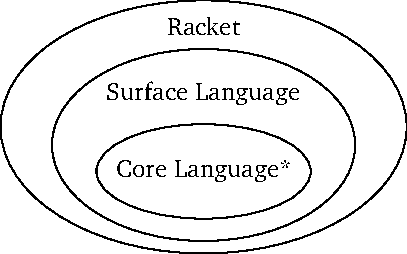
\includegraphics{images/language-hierarchy.pdf}
  \caption{The hierarchy of languages. The Core Language is the language analyzed by our analyzer, which includes only the essential features of higher-order programming. The Surface Language is the language in which we write our examples and tests—it includes more features for convenience. The Core Language is a subset of the Surface Language (* except for the labels on each program point), and the Surface Language is a subset of Racket.}
  \label{figure:language-hierarchy}
\end{figure}

\subsection{Core Language (\texttt{ᶜ})}
\label{section:core-language}

The Core Language is the language analyzed by our analyzer. To keep the analyzer as simple as possible, the Core Language includes only the essential features of higher-order programming:

\begin{description}
  \item [Function.] The only kind of value is the function, for example, \texttt{(λ (x) x)} is a function that simply returns its argument (the identity function). A function may receive only one argument (unary function).
  \item [Call.] The only kind of operation is the function call, for example, \texttt{((λ (x) x) (λ (y) y))} is a call of the function \texttt{(λ (x) x)} (the identity function) with the argument \texttt{(λ (y) y)} (which happens to be another identity function).
  \item [Variable Reference.] Variables may only be referenced after they are defined, for example, the fragment \texttt{(λ (x) \highlight{x})} is a program in the Core Language because the variable \texttt{x} is only referenced in \texttt{\highlight{x}} after it is defined in \texttt{(λ (x) \_\_\_)}, but the fragment \texttt{(λ (x) \highlight{y})} is not a program in the Core Language because the variable \texttt{\highlight{y}} is undefined. We say that \texttt{\highlight{x}} is a \emph{closed variable reference} and that the former fragment is \emph{closed}, but that \texttt{\highlight{y}} is an \emph{open variable reference} and that the latter fragment is \emph{open}. Only closed fragments may be programs in the Core Language.
\end{description}

Our analyzer must disambiguate between fragments that look the same, so we label each program point with a unique integer. For example, in the program \texttt{((λ (x) x) (λ (x) x))}) the two fragments \texttt{(λ (x) x)} look the same, but the labels disambiguate them: \texttt{((((λ (x) (x . 0)) . 1) ((λ (x) (x . 2)) . 3)) . 4)}.

The grammar for the Core Language is in Figure~\ref{figure:core-language-grammar} (refer to \url{http://matt.might.net/articles/grammars-bnf-ebnf/} to learn how to read a grammar).

\begin{figure}[h]
  \centering
  \begin{tabular}{rcll}
             \(e\) & ::= & \(f\) | \(c\) | \(r\)                 & Expressions         \\
             \(f\) & ::= & \texttt{((λ (\(x\)) \(e\)) . \(ℓᶠ\))} & Functions           \\
             \(c\) & ::= & \texttt{((\(e\) \(e\)) . \(ℓᶜ\))}     & Calls               \\
             \(r\) & ::= & \texttt{(\(x\) . \(ℓʳ\))}             & Variable References \\
            \(ℓᵉ\) & ::= & \(ℓᶠ\) | \(ℓᶜ\) | \(ℓʳ\)              & Labels              \\
    \(ℓᶠ, ℓᶜ, ℓʳ\) & ::= & «Disjoint Sets of Integers»           &                     \\
             \(x\) & ::= & «Identifiers»                         & Identifiers         \\
  \end{tabular}
  \caption{Core Language’s grammar.}
  \label{figure:core-language-grammar}
\end{figure}

Identifiers (\(x\)) in the Core Language have the same form as identifiers in Racket.

The grammar differentiates the labels for different kinds of expression (\(ℓᶠ\), \(ℓᶜ\), and \(ℓʳ\)). We do this because we want the structures in our analyzer to be as compact as possible, so we let a label stand for an expression when we are interested only in its identity rather than in its form, but we must be able to distinguish between the different kinds of expressions. For example, in Step 2~(§~\ref{section:step-2--introduce-time-stamps}) we define something called \emph{time stamps} (\(t\)) in terms of call sites (\(c\)) and we use their labels (\(ℓᶜ\)) because we are interested only in their identities rather than in what function was called or in what argument was passed to it—the different kinds of labels prevent other kinds of expressions (those represented by \(ℓᶠ\) and \(ℓʳ\)) from occurring in time stamps.

When we are dealing with multiple languages, we use the superscript \(ᶜ\) to represent the Core Language and avoid ambiguity. For example, when we are defining the compiler from the Surface Language to the Core Language~(§~\ref{section:compiling-the-surface-language-into-the-core-language}) we represent an expression in the Core Language as \(eᶜ\).

In technical terms, the Core Language is something called the \emph{labeled call-by-value statically-scoped \(λ\)-calculus}.

\subsection{Surface Language (\texttt{ˢ})}
\label{section:surface-language}

The Surface Language is the language in which we write our examples and tests. For our convenience, the Surface Language includes more features than the Core Language~(§~\ref{section:core-language}), but before our analyzer can analyze a program in the Surface Language, it must be compiled~(§~\ref{section:compiling-the-surface-language-into-the-core-language}) to the Core Language. The Surface Language is a subset of Racket which supports the forms defined in Figure~\ref{figure:surface-language-grammar}.

\begin{figure}[h]
  \centering
  % \begin{tabular}{rcll}
  % \end{tabular}
  \caption{Surface Language’s grammar.}
  \label{figure:surface-language-grammar}
\end{figure}

\begin{itemize}
  \item Architecture
  \item  We achieve this simplicity in presentation by making the analyzed language small and by using relatively straightforward programming techniques, not by compromising on features: the resulting program analyzer is the state-of-the-art.
  \item Surface language \& Core language §~\ref{section:compiling-the-surface-language-into-the-core-language}
  \item Reduce~(\(⇒\)) \& Lift~(\(⇑\))
  \item Draw a picture of the square.
  \item In many cases \(⇑\) is more complicated than \(⇒\), justifying our philosophical claim that analyses should be presented doing the full circle (see § on the philosophy of investigating program analysis).
  \item There are other clients beyond \(⇑\), for example, dependency analysis, environment analysis, and so forth
  \item In the abstract interpreter at Step~10, the only part of the process that may not terminate is decoding. \(⇓\), \(⇒\), \(⇑\) and evaluating the resulting Racket S-expression are all guaranteed to terminate. In the Steps~0–6, \(⇒\) may not terminate, but \(⇓\), and \(⇑\) always do.
  \item We only show the parts that change between the steps
  \item Represent tuples with lists, associations (mappings) with hashes, and sets with Racket sets.
  \item Give examples of machine dumps and lifted expressions for each step.
  \item Read the code by diffing the steps.
  \item Soundness proof = ADI + Allocation Characterizes Polyvariance
\end{itemize}

\begin{itemize}
  \item High-Level View
  \item Finitize the space \& check for cycles
  \item Finitize the space using the AAM trick: (1)~removing the recursion from the data structures (figure with diagram of grammars, one including a cycle and another not including it); and (2)~finitizing the space of addresses.
  \item Briefly describe each step.
\end{itemize}

\begin{itemize}
  \item Regarding test programs:
  \item Programs like \texttt{sat} are common in the program analysis literature, but they’re a bad example because they include the data literally in the source code. That’s unrealistic, usually we’d want to compute on data given by the user, and to be capable of compute on data in general. The problem is that a program analyzer may be over-specializing to solve satisfiability for that one formula. Also, it’s only because of this that we’re exponential (and so are many other exponential analysis). This may be like saying that OCaml’s typechecker is exponential: yes, it is, but nobody cares, because in practice it’s OK. If we analyze a more realistic SAT-solver, then the formula is given as user input and it may contain any number of variables, so we can’t call \texttt{try} a fixed number of times. When that happens, we’re writing a recursive function, on which our context model bails early and doesn’t lose time.
  \item The test programs never rely on something buried in the encoding to show the difference between steps, or to make statements about running time. For example, we never rely on addition or properties of numbers. We always bring out the imprecisions to the source of the surface program, in such a way that the result we’re showing would occur even if the analysis was defined over a bigger language instead of relying on encodings, a bigger language that included numbers and functions with multiple arguments as first-class citizens, for example.
\end{itemize}

\section{Step 0: Base Interpreter}
\label{section:step-0--base-interpreter}

\begin{itemize}
  \item Ground truth
  \item Substitution-based \& Big-step.
  \item Meta-circular (like the original LISP definition)
\end{itemize}

\subsection{Reduce~(\(⇒\))}

\begin{Verbatim}
;; ⇒ : e → f
(define (⇒ e)

  ;; substitute : e x f → e
  (define (substitute e xˢ f)
    (match e
      [`((λ (,x) ,eᵇ) . ,ℓᶠ) #:when (equal? xˢ x) e]
      [`((λ (,x) ,eᵇ) . ,ℓᶠ) `((λ (,x) ,(substitute eᵇ xˢ f)) . ,ℓᶠ)]
      [`((,eᶠ ,eᵃ) . ,ℓᶜ) `((,(substitute eᶠ xˢ f) ,(substitute eᵃ xˢ f)) . ,ℓᶜ)]
      [`(,(? symbol? x) . ,ℓʳ) #:when (equal? xˢ x) f]
      [`(,(? symbol? x) . ,ℓʳ) e]))

  (match e
    [`((λ (,x) ,eᵇ) . ,ℓᶠ) e]
    [`((,eᶠ ,eᵃ) . ,ℓᶜ)
     (match-define fᶠ (⇒ eᶠ))
     (match-define fᵃ (⇒ eᵃ))
     (match-define `((λ (,x) ,eᵇ) . ,ℓᶠ) fᶠ)
     (⇒ (substitute eᵇ x fᵃ))]))
\end{Verbatim}

\begin{itemize}
  \item We don’t need a clause for when reduction encounters a variable, because it’ll have been substituted by then (our programs must be closed!)
  \item Because of substitution, the labels in the result may be repeated, tracing back to the original program. For example, \texttt{((λ (f) (thunk (f f))) (λ (x) x))}
  \item This is similar to how kids do arithmetic in grade school
\end{itemize}

\subsection{Lift~(\(⇑\))}

\begin{Verbatim}
;; ⇑ : f → Racket S-Expression
(define (⇑ f)
  ;; ↑ : e → Racket S-Expression
  (define (↑ e)
    (match e
      [`((λ (,x) ,eᵇ) . ,ℓᶠ) `(λ (,x) ,(↑ eᵇ))]
      [`((,eᶠ ,eᵃ) . ,ℓᶜ) `(,(↑ eᶠ) ,(↑ eᵃ))]
      [`(,(? symbol? x) . ,ℓʳ) x]))
  (↑ f))
\end{Verbatim}

\begin{itemize}
  \item Remove labels.
  \item The definition of \(↑\) may seem superfluous now, but it highlights the change in input type (\(f\) in \(⇑\) vs. \(e\) in \(↑\)), and it’ll make more sense in the next steps, in which \(↑\) will have more arguments than just the expression \(e\).
\end{itemize}

\subsection{Evaluate (\(eval\))}

\begin{Verbatim}
;; eval : eˢ decoder → Racket Value
(define (eval e [decode identity]) (decode (racket:eval (⇑ (⇒ (⇓ e))))))
\end{Verbatim}

\subsection{Tests}

\section{Step 1: Environment-Based Interpreter}

\begin{itemize}
  \item Evaluator (\(eval\)) \& tests remain the same, because the semantics is the same; only \(⇒\) \& \(⇑\) change
  \item We introduce some Machinery to help in evaluation; the user is never supposed to see this machinery (and this is a major contribution of our work, because usually papers stop short by just showing the result of the machinery and looking at its intrinsic properties!)
\end{itemize}

\subsection{Machinery}

\begin{tabular}{rcll}
  \(v\) & ::= & \(⟨f, ρ⟩\)       & Values       \\
  \(ρ\) & ::= & \([x ↦ v, ...]\) & Environments \\
\end{tabular}

\begin{itemize}
  \item Values are called \emph{closures}.
\end{itemize}

\subsection{Reduce~(\(⇒\))}

\begin{Verbatim}
;; ⇒ : e → ◊highlight«¹v»
(define (⇒ e)

  ;; → : e ◊highlight«³ρ» → ◊highlight«¹v»
  (define (◊highlight«²→» e ◊highlight«³ρ»)
    (match e
      [`((λ (,x) ,eᵇ) . ,ℓᶠ) ◊highlight«⁷`(,e ,ρ)»]
      [`((,eᶠ ,eᵃ) . ,ℓᶜ)
       (match-define ◊highlight«⁸vᶠ» (→ eᶠ ◊highlight«⁶ρ»))
       (match-define ◊highlight«⁹vᵃ» (→ eᵃ ◊highlight«⁶ρ»))
     ◊highlight«¹⁰(match-define `(((λ (,x) ,eᵇ) . ,ℓᶠ) ,ρᶠ) vᶠ)»
      ◊highlight«⁵(match-define ρᶠ⁺ˣ (hash-set ρᶠ x vᵃ))»
     ◊highlight«¹¹(→ eᵇ ρᶠ⁺ˣ)»]
    ◊highlight«¹²[`(,(? symbol? x) . ,ℓʳ) (hash-ref ρ x)]»))

  (→ e ◊highlight«⁴(hash)»))
\end{Verbatim}

\begin{itemize}
  \item (1)~The function \(⇒\) returns a value \(v\), as opposed to a function \(f\)
  \item We don’t perform substitutions right away, so we remove \(substitute\).
  \item (2)~We have an auxiliary function \(→\) (3)~to hold the current environment \(ρ\), (4)~which starts empty and (5)~is augmented with mappings from formal parameters to actual arguments; (6)~everywhere else it is just threaded unchanged.
  \item In ADI, the environment \(ρ\) is kept with a \emph{Reader} monad.
  \item (7)~When we encounter a function, we produce a value \(v\) by pairing the function with the current environment \(ρ\), because a function must remember the non-locals from where it was defined.
  \item When we encounter a call, we start the same way as before in the base interpreter. (8)~We evaluate the expression at the function position \(eᶠ\) and (9)~the expression at the argument position \(eᵃ\). But instead of substituting the argument in the function body, (10)~we recover the environment \(ρᶠ\) from where the function was defined, because we want the non-locals to refer to there. Next, (5)~we extend the environment \(ρᶠ\) with a mapping from the formal parameter \(x\) to the actual argument \(vᵃ\), so that occurrences of \(x\) in the body \(eᵇ\) can be looked up. Finally, (11)~reduction proceeds in the body \(eᵇ\) with this extended environment \(ρᶠ⁺ˣ\).
  \item (12)~When we encounter a variable, we look it up in the environment.
  \item Now the labels don’t repeat, because we’re delaying substitution.
  \item This is similar to how a debugger works.
\end{itemize}

\subsection{Lift~(\(⇑\))}

\begin{Verbatim}
;; ⇑ : ◊highlight«¹v» → Racket S-Expression
(define (⇑ ◊highlight«¹v»)
 ◊highlight«²(match-define `(,f ,ρ) v)»
  ;; ↑ : e ◊highlight«³{x, ...}» → Racket S-Expression
  (define (↑ e ◊highlight«³x*»)
    (match e
      [`((λ (,x) ,eᵇ) . ,ℓᶠ) `(λ (,x) ,(↑ eᵇ ◊highlight«⁵(set-add x* x)»))]
      [`((,eᶠ ,eᵃ) . ,ℓᶜ) `(,(↑ eᶠ ◊highlight«⁶x*») ,(↑ eᵃ ◊highlight«⁶x*»))]
      [`(,(? symbol? x) . ,ℓʳ) ◊highlight«⁷#:when (set-member? x* x)» ◊highlight«⁸x»]
      [`(,(? symbol? x) . ,ℓʳ) (◊highlight«¹⁰⇑» ◊highlight«⁹(hash-ref ρ x)»)]))
  (↑ f ◊highlight«⁴(set)»))
\end{Verbatim}

\begin{itemize}
  \item (1)~\(⇑\) receives a value \(v\) as argument, as opposed to just a function \(f\) like in Step~0. This matches the change in return type in \(⇒\) (see (1) in the previous subsection).
  \item (2)~We deconstruct the value \(v\) and make its environment \(ρ\) available for the auxiliary function \(↑\).
  \item (3)~The auxiliary function \(↑\) receives as argument a set of bound variables \(x*\). (4)~To begin with, the set of bound variables is empty. (5)~We extend the set of bound variables when we enter a function body. (6)~In all other cases we just thread the set of bound variables unmodified.
  \item In ADI terms, the set of bound variables \(x*\) would be a \emph{Reader} monad.
  \item (7)~When we find a variable, we first check if it’s bound. (8)~If it is, then we leave it unchanged. (9)~If it isn’t, then this variable is a non-local and its meaning is looked up in the environment. (10)~The result of looking up a variable in the environment is a value, which itself must be lifted.
\end{itemize}

\section{Step 2: Introduce Time Stamps}
\label{section:step-2--introduce-time-stamps}

\begin{itemize}
  \item We introduce time stamps to use on the next step. So we compute it, keep it around, and do nothing with it yet.
  \item Time Stamps are also known as contours.
  \item Only reduce~(\(⇒\)) changes, because the semantics (so tests don’t change) and the structure of return types are the same (so \(⇑\) \& \(eval\) don’t change).
  \item Time stamps are unique throughout the evaluation of the program. This is important because we use the time stamps as part of the addresses. The uniqueness stems from each call site only being visited once under a certain time stamp, and even when the time stamps fork in \texttt{eᶠ} and \texttt{eᵃ}, their children will inductively be the same, because \texttt{eᶠ} and \texttt{eᵃ} can’t be the same call site.
  \item In fact, the main reason why we introduce time stamps is as a source of freshness.
\end{itemize}

\subsection{Machinery}

\begin{tabular}{rcll}
  \(t\) & ::= & \([ℓᶜ, ...]\) & Time Stamps \\
\end{tabular}

\subsection{Reduce~(\(⇒\))}

\begin{Verbatim}
;; ⇒ : e → v
(define (⇒ e)

  ;; → : e ρ ◊highlight«¹t» → v
  (define (→ e ρ ◊highlight«¹t»)
    (match e
      [`((λ (,x) ,eᵇ) . ,ℓᶠ) `(,e ,ρ)]
      [`((,eᶠ ,eᵃ) . ,ℓᶜ)
      ◊highlight«³(match-define tᵉ (cons ℓᶜ t))»
       (match-define vᶠ (→ eᶠ ρ ◊highlight«⁴tᵉ»))
       (match-define vᵃ (→ eᵃ ρ ◊highlight«⁴tᵉ»))
       (match-define `(((λ (,x) ,eᵇ) . ,ℓᶠ) ,ρᶠ) vᶠ)
       (match-define ρᶠ⁺ˣ (hash-set ρᶠ x vᵃ))
       (→ eᵇ ρᶠ⁺ˣ ◊highlight«⁴tᵉ»)]
      [`(,(? symbol? x) . ,ℓʳ) (hash-ref ρ x)]))

  (→ e (hash) ◊highlight«²empty»))
\end{Verbatim}

\begin{itemize}
  \item (1)~The \(→\) function receives an additional argument for the time stamp \(t\). (2)~To begin with, the time stamp is empty. (3)~When we encounter a call site, we \emph{tick} the clock and create a new time stamp. (4)~This new time stamp is passed to the recursive calls.
  \item In ADI terms, this is the \emph{Reader} monad.
  \item We use labels \(ℓ⁽ᵉ⁺ᶠ⁺ᶜ⁺ʳ⁾\) to represent expressions when we are interested only in their identity, not their contents.
\end{itemize}

\section{Step 3: Introduce Indirection Through the Store}

\begin{itemize}
  \item Evaluate (\(eval\)) \& the tests stay the same, because the semantics is still the same. But both \(⇒\) and \(⇑\) change.
\end{itemize}

\subsection{Machinery}

\begin{tabular}{rcll}
  \(¢\) & ::= & \(⟨v, σ⟩\)       & Results      \\
  \(ρ\) & ::= & \([x ↦ a, ...]\) & Environments \\
  \(σ\) & ::= & \([a ↦ v, ...]\) & Stores       \\
  \(a\) & ::= & \(⟨ℓᶠ, t⟩\)      & Addresses    \\
\end{tabular}

\begin{itemize}
  \item We must allocate new addresses every time, to guarantee that keys in the store don’t clash.
  \item In CPS, like in Shivers’ original \(k\)-CFA presentation, it’s trivial that the time stamps—and therefore the addresses—are unique. But in our language that isn’t so trivial, because the time stamps \emph{fork} during evaluation. There’s a whole argument to be made about why the freshness of addresses holds. The core of the argument has to do with evaluation never revisiting a call site under the same time stamp. A more complete presentation of this argument is found on Zach’s dissertation and on Dr.~Scott’s paper on test-case generation.
  \item The \(f\) in \(a\) is superfluous for now, because the time stamp \(t\) is already unique for each call site we encounter. But including \(f\) in \(a\) increases analysis precision in later steps for recursive functions that create closures. For example, \texttt{Ω/creating-closures}’s result would be imprecise under Step~7 if it were not for \(f\).
  \item Traditionally, people don’t add the function identity \(ℓᶠ\) to the address \(a\), but the variable it binds \(x\). This requires alphatising the program to improve precision. We’d want to include \(x\) in \(a\) if we were to support functions with multiple arguments (uncurried); under the assumption that the multiple arguments must have different names.
  \item Why is it always allocating new timestamps? Because the only control flow operation is calling functions so the same expression cannot be visited more than once with the same timestamp.
\end{itemize}

\subsection{Reduce~(\(⇒\))}

\begin{Verbatim}
;; ⇒ : e → ◊highlight«¹¢»
(define (⇒ e)

  ;; → : e ρ ◊highlight«²σ» t → ◊highlight«¹¢»
  (define (→ e ρ ◊highlight«²σ» t)
    (match e
      [`((λ (,x) ,eᵇ) . ,ℓᶠ) `((,e ,ρ) ,σ)]
      [`((,eᶠ ,eᵃ) . ,ℓᶜ)
       (match-define tᵉ (cons ℓᶜ t))
       (match-define ¢ᶠ (◊highlight«⁷→» eᶠ ρ σ tᵉ))
       (match-define ¢ᵃ (◊highlight«⁶→» eᵃ ρ ◊highlight«⁵(second ¢ᶠ)» tᵉ))
       (match-define vᶠ (first ¢ᶠ))
       (match-define vᵃ (first ¢ᵃ))
       (match-define `(((λ (,x) ,eᵇ) . ,ℓᶠ) ,ρᶠ) vᶠ)
       (match-define σᶠ⁺ᵃ (second ¢ᵃ))
      ◊highlight«⁸(match-define a `(,ℓᶠ ,tᵉ))»
       (match-define ρᶠ⁺ˣ (hash-set ρᶠ x a))
      ◊highlight«⁴(match-define σᶠ⁺ᵃ⁺ˣ (hash-set σᶠ⁺ᵃ a vᵃ))»
       (→ eᵇ ρᶠ⁺ˣ ◊highlight«⁹σᶠ⁺ᵃ⁺ˣ» tᵉ)]
      [`(,(? symbol? x) . ,ℓʳ) `(,(hash-ref σ (hash-ref ρ x)) ,σ)]))

  (→ e (hash) ◊highlight«³(hash)» empty))
\end{Verbatim}

\begin{itemize}
  \item (1)~\(⇒\) returns a result \(¢\) instead of just a value \(v\). The result \(¢\) includes a store \(σ\) with which we may look up the addresses \(a\) that we fetch from the environment.
  \item (2)~\(→\) has a store \(σ\) as an extra argument. (3)~To begin with, \(σ\) is empty, (4)~and we extend it when we encounter a function application. The other recursive calls to \(→\) don’t just thread \(σ\) like they do for the environment \(ρ\) and the time stamp \(t\), because the (5)~extensions to \(σ\) from (6)~one call are available on (7)~the next. When we encounter a function call, we \emph{fork} and call \(→\) recursively twice to reduce the expressions at (7)~function position and (6)~argument position; in this occasion, while \(ρ\) and \(t\) are \emph{forked} as well, (5)~\(σ\) grows monotonically. This is necessary because values hold \(ρ\), but they don’t hold \(σ\), so we couldn’t retrieve \(σ\) like we retrieve \(ρ\) when we’re about to enter a function body.
  \item In ADI terms, the store \(σ\) is the \emph{State} monad.
  \item When we encounter a function application, (4)~we must extend the store, (8)~so allocate an address based on the function \(f\) we are about to enter (represented in the code by \(ℓᶠ\)), and the current time stamp \(tᵉ\). (9)~We enter the function body with this extended store \(σᶠ⁺ᵃ⁺ˣ\).
  \item It is common to extract the allocation in (8) into its own function, but we won’t, for simplicity
\end{itemize}

\subsection{Lift~(\(⇑\))}

\begin{Verbatim}
;; ⇑ : ◊highlight«¹¢» → Racket S-Expression
(define (⇑ ◊highlight«¹¢»)

 ◊highlight«³;; ⇑/a : a → Racket S-Expression (Identifier)»
  ◊highlight«(define (⇑/a a) (string->symbol (~a a)))»

  ;; ◊highlight«⁴⇑/v» : v → Racket S-Expression
  (define (◊highlight«⁴⇑/v» v)
    (match-define `(,f ,ρ) v)
    ;; ↑ : e {x, ...} → Racket S-Expression
    (define (↑ e x*)
      (match e
        [`((λ (,x) ,eᵇ) . ,ℓᶠ) `(λ (,x) ,(↑ eᵇ (set-add x* x)))]
        [`((,eᶠ ,eᵃ) . ,ℓᶜ) `(,(↑ eᶠ x*) ,(↑ eᵃ x*))]
        [`(,(? symbol? x) . ,ℓʳ) #:when (set-member? x* x) x]
        [`(,(? symbol? x) . ,ℓʳ) (◊highlight«⁵⇑/a» (hash-ref ρ x))]))
    (↑ f (set)))

  (match-define `(,v ,σ) ¢)
 ◊highlight«²`(letrec (,@(for/list ([(a v) (in-hash σ)]) `[,(⇑/a a) ,(⇑/v v)]))»
     ,(⇑/v v)))
\end{Verbatim}

\begin{itemize}
  \item (1)~The argument for \(⇑\) is a result \(¢\), as opposed to just a value \(v\).
  \item (2)~We lift the store \(σ\) with \texttt{letrec}, which makes all the bindings for the non-locals recursively available to one another.
  \item (3)~\(⇑/a\) lifts addresses as identifiers, which we use as bindings for the non-locals in the \texttt{letrec}. We just convert the S-expression that is the address into a symbol, which produces identifiers with strange names, for example, \texttt{|(2 (11 3))|}, in which \texttt{|} delimit an identifier.
  \item (4)~\(⇑/v\) is almost the same as the previous implementation of \(⇑\), except that (5)~we modify it to use \(⇑/a\) as opposed to \(⇑\) when lifting the contents fetched from the environment \(ρ\), because they changed their type.
\end{itemize}

\section{Step 4: Introduce Nondeterminism in the Store}

\subsection{Machinery}

\begin{tabular}{rcll}
  \(£\) & ::= & \(\{¢, ...\}\)   & Result Sets      \\
  \(¢\) & ::= & \(⟨d, σ⟩\)       & Results          \\
  \(d\) & ::= & \(\{v, ...\}\)   & Denotable Values \\
  \(σ\) & ::= & \([a ↦ d, ...]\) & Stores           \\
\end{tabular}

\begin{itemize}
  \item We reify nondeterministic choices with sets.
  \item We introduce two points of nondeterminism: in results \(¢\) \& stores \(σ\), and in the result sets. The first point is because we want to support nondeterminism in values, which is why we introduce denotable values \(d\). The second is because each time we encounter nondeterministic values, we \emph{fork} the universe and explore each choice independently. More importantly, we do not share stores \(σ\) among these universes (we do not widen the store) (but we could, see §~store widening). So the result of the explorations will be multiple results \(¢\), which we collect in result sets \(£\).
  \item Both \(d\) and \(£\) are guaranteed to be singletons for the time being, because we have an allocator of addresses that produces fresh addresses every time. But start on the next step, the sets may no longer be singletons.
  \item We can only have multiple values in \(d\) as the result of merging in the store \(σ\), and we can only have multiple values in \(£\) as the result of exploring different universes because some \(d\) isn’t a singleton.
  \item The stores \(σ\) are maps of sets, or \emph{multi-maps}.
  \item \emph{Denotable values} are also called \emph{flow sets} in the literature.
  \item At this step, it’s common in the literature to start notating \emph{all} components with hats (\(\hat{~}\)), but we won’t do that here to make things more readable.
\end{itemize}

\subsection{Reduce~(\(⇒\))}

\begin{Verbatim}
;; ⇒ : e → ◊highlight«¹£»
(define (⇒ e)

  ;; → : e ρ σ t → ◊highlight«¹£»
  (define (→ e ρ σ t)
    (match e
      [`((λ (,x) ,eᵇ) . ,ℓᶠ) (◊highlight«³set» `(,(◊highlight«²set» `(,e ,ρ)) ,σ))]
      [`((,eᶠ ,eᵃ) . ,ℓᶜ)
       (match-define tᵉ (cons ℓᶜ t))
       (◊highlight«⁹apply»
        ◊highlight«⁹set-union»
        (◊highlight«⁷for*/list» ([¢ᶠ (in-set (→ eᶠ ρ σ tᵉ))]
                    [¢ᵃ (in-set (→ eᵃ ρ (second ¢ᶠ) tᵉ))]
                    [vᶠ (in-set ◊highlight«⁸(first ¢ᶠ)»)]
                    [vᵃ (in-set ◊highlight«⁸(first ¢ᵃ)»)])
          (match-define `(((λ (,x) ,eᵇ) . ,ℓᶠ) ,ρᶠ) vᶠ)
          (match-define σᶠ⁺ᵃ (second ¢ᵃ))
          (match-define a `(,ℓᶠ ,tᵉ))
          (match-define ρᶠ⁺ˣ (hash-set ρᶠ x a))
          (match-define σᶠ⁺ᵃ⁺ˣ (◊highlight«⁵hash-union» σᶠ⁺ᵃ (hash a (set vᵃ)) #:combine ◊highlight«⁶set-union»))
          (→ eᵇ ρᶠ⁺ˣ σᶠ⁺ᵃ⁺ˣ tᵉ)))]
      [`(,(? symbol? x) . ,ℓʳ) (◊highlight«⁴set» `(,(hash-ref σ (hash-ref ρ x)) ,σ))]))

  (→ e (hash) (hash) empty))
\end{Verbatim}

\begin{itemize}
  \item (1)~Both \(⇒\) and its auxiliary function \(→\) return results sets \(£\), as opposed to just results \(¢\).
  \item We do almost the same as before when we encounter a function, but (2)~we wrap the value \(v\) in a set to form a denotable value \(d\), and (3)~we wrap the whole result \(¢\) in a set to form a result set \(£\).
  \item We do almost the same as before when we encounter a variable reference, but (4)~we wrap the result \(¢\) in a set to form a result set \(£\). We don’t need to wrap values in sets, as we do in (2), because the store \(σ\) returns a denotable value \(d\).
  \item To extend the stores \(σ\) with new bindings, we no longer overwrite using \texttt{hash-set}. If a key is repeated in the store, we union the denotable values (which are sets) with a combination of (5)~\texttt{hash-union} and (6)~\texttt{set-union}.
  \item In the literature, this union operations is often notated \(⊔\).
  \item (7)~To explore different universes of values nondeterministically, we use \texttt{for*/list}, which creates a series of nested \texttt{for} loops (8)~iterating over the denotable values (sets of values).
  \item (9)~We combine the result sets from all the universes with the \texttt{apply set-union} idiom.
  \item For this step, sets are guaranteed to be singletons (see argument in the previous subsection), and we could have used this invariant to simplify this step a lot. First, \texttt{hash-set} would have worked the same as \texttt{hash-union}. Second, we wouldn’t need to \emph{fork} the universe with \texttt{for*/list}. Third, we wouldn’t need to union the results with the \texttt{apply set-union} idiom. But starting on the next section sets may not be singletons, so it’s better to prepare for nondeterminism in this step.
  \item In ADI’s terms, this is the \emph{Nondeterminism} monad.
\end{itemize}

\subsection{Lift~(\(⇑\))}

\begin{Verbatim}
;; ⇑ : ◊highlight«¹£» → Racket S-Expression
(define (⇑ ◊highlight«¹£»)

  ;; ◊highlight«⁴⇑/¢» : ¢ → Racket S-Expression
  (define (◊highlight«⁴⇑/¢» ¢)
    (match-define `(,d ,σ) ¢)
    `(◊highlight«⁵letrec» (,@(for/list ([(a d) (in-hash σ)])
                ◊highlight«¹⁰(define xᵏ (gensym))»
                  `[,(⇑/a a)
                    (◊highlight«⁷thunk» (◊highlight«⁹shift» ◊highlight«¹⁰,xᵏ» (◊highlight«¹¹set-union ,@(for/list ([v (in-set d)])»
                                                         ◊highlight«¹²`(,xᵏ ,(⇑/v v))»))))]))
       ◊highlight«⁶(set ,@(set-map d ⇑/v))»))

  ;; ⇑/a : a → Racket S-Expression (Identifier)
  (define (⇑/a a) (string->symbol (~a a)))

  ;; ⇑/v : v → Racket S-Expression
  (define (⇑/v v)
    (match-define `(,f ,ρ) v)
    ;; ↑ : e {x, ...} → Racket S-Expression
    (define (↑ e x*)
      (match e
        [`((λ (,x) ,eᵇ) . ,ℓᶠ) `(λ (,x) ,(↑ eᵇ (set-add x* x)))]
        [`((,eᶠ ,eᵃ) . ,ℓᶜ) `(,(↑ eᶠ x*) ,(↑ eᵃ x*))]
        [`(,(? symbol? x) . ,ℓʳ) #:when (set-member? x* x) x]
        [`(,(? symbol? x) . ,ℓʳ) `◊highlight«⁸(»,(⇑/a (hash-ref ρ x))◊highlight«)»]))
    (↑ f (set)))

  `(begin ◊highlight«¹³(require (only-in racket/control shift))»
          (◊highlight«³set-union» ◊highlight«²,@(for/list ([¢ (in-set £)]) (⇑/¢ ¢))»)))
\end{Verbatim}

\begin{itemize}
  \item (1)~To match the output of \(⇒\), the \(⇑\) function accepts result sets \(£\) as inputs, as opposed to results \(¢\).
  \item (2)~We lift result sets \(£\), by first lifting each result \(¢\) with \(⇑/¢\), and (3)~then combining the outputs.
  \item (4)~The \(⇑/¢\) function is similar to the implementation of \(⇑\) from the previous step; for example, (5)~it uses \texttt{letrec} to lift the store \(σ\). But \(⇑/¢\) has changed in a few places.
  \item (6)~First, \(⇑/¢\) produces a Racket S-expression that generates a set of values lifted with \(⇑/v\). This matches the change in machinery (see corresponding §) in which \(¢\) contain denotable values \(d\) instead of values \(v\).
  \item Second, \(⇑/¢\) must handle the change in \(σ\), which maps addresses \(a\) to denotable values \(d\) instead of values \(v\). But this case is more complicated than the one in~(6), because the store \(σ\) may be looked up from within a lifted function. For example, the result of \(⇑/¢\) may be \texttt{(letrec ([a@1 \_\_\_]) (set (λ (\_) a@1)))}, and the non-local variable \texttt{a@1} may be looked up when the function is applied from within a decoder (see §~appendix on decoders) at the \(eval\) (see §~below) step. But the decoders work over values, not sets of them, so we cannot use sets like we did in~(6).
  \item We could convert the decoders so that they work over sets of values using the \texttt{apply set-union} idiom, for example, we could convert \(decode/boolean\) into \(decode*/boolean\):
        \begin{Verbatim}
(define (decode/boolean e) ((e #t) #f))
(decode/boolean (λ (a) (λ (b) a))) ;; ⇒ #t
(define (decode*/boolean e)
  ◊highlight«(apply set-union»
         ◊highlight«(for/list ([e² (in-set (apply set-union»
                                       ◊highlight«(for/list ([e¹ (in-set e)])»
                                         (e¹ #t)◊highlight«)))])»
           (e² #f)◊highlight«))»)
(decode*/boolean ◊highlight«(set »(λ (a) ◊highlight«(set »(λ (b) ◊highlight«(set »a◊highlight«)»)◊highlight«)»)◊highlight«)») ;; ⇒ ◊highlight«(set »#t◊highlight«)»
        \end{Verbatim}
        But these conversions are tedious to carry out, prone to errors, and don’t scale well for more elaborate data types.
  \item In most base languages, global program transformations like the decoder conversion proposed above would be our only choice. But in Racket there’s a feature that solves our problem in a straightforward manner: delimited continuations. In particular, we use \texttt{shift/reduce} à la Abstracting Control~(Danvy 1990) to simulate nondeterminism in choosing a \(v\) from \(d\).
  \item (7)~We do not want to always explore the cartesian product of each \(v\) in each \(d\), because that would be expensive. So we start to lift the \(d\) in the \texttt{letrec} representing the store \(σ\) by wrapping it in a \emph{thunk}. (8)~We force this thunk when we find a non-local variable.
  \item Next, (9)~we use \texttt{shift} to capture the current (delimited) continuation (10)~into a fresh variable \(xᵏ\). The \texttt{reset} corresponding to this \texttt{shift} appears on \(eval\) (see § below) and wraps \emph{around} the decoder. From the decoder’s perspective, it can work with a single value.
  \item (11)~Finally, we iterate over each \(v\) in \(d\) and accumulate the sets of results of (12)~invoking continuation captured in \(xᵏ\) with the lifted \(v\).
  \item (13)~We have to require the \texttt{shift} operator.
\end{itemize}

\subsection{Evaluate (\(eval\))}

\begin{Verbatim}
;; eval : eˢ decoder → Racket Value
(define (eval e [decode identity])
  (◊highlight«⁴apply set-union»
        ◊highlight«¹(for/list ([eʳ (in-set» (racket:eval (⇑ (⇒ (⇓ e)))))])
           (◊highlight«⁵reset» (◊highlight«³set» (◊highlight«²decode» eʳ))))))
\end{Verbatim}

\begin{itemize}
  \item (1)~The \(eval\) function has to iterate over the set of values generated by the lifted Racket S-expression, (2)~calling the decoder for each of them.
  \item (3)~The decoded values are wrapped in (singleton) sets, which (4)~are aggregated with the \texttt{apply set-union} idiom.
  \item (5)~The \texttt{reset} corresponding to the \texttt{shift} that we introduced in the lifted S-expression (see §~above) goes around the (singleton) set, which guarantees that calling the continuation captured in \(xᵏ\) produces sets.
\end{itemize}

\subsection{Tests}

\begin{itemize}
  \item The behavior of the evaluator in this step is the same, but its return type has changed: it returns result \emph{sets}, so we must modify the tests accordingly, for example:
        \begin{Verbatim}
;; Before
(check-equal? (eval application decode/boolean) #t)
;; After
(check-equal? (eval application decode/boolean) (set #t))
        \end{Verbatim}
\end{itemize}

\section{Step 5: Finitize the Space of Addresses}
\label{section:step-5--finitize-the-space-of-addresses}

\begin{itemize}
  \item We finally accomplish the first of two goals towards an analysis: we finitize the space that the analysis may explore by finitizing the possible values \(v\). The second goal is to detect when we’re revisiting work, and stop, but to do that in a manner that remains sound. This second goal is the subject of the next steps.
  \item Only reduce~(\(⇒\)) changes, because lift~(\(⇑\)) and \(eval\) are already prepared it to handle nondeterminism, but this affects the tests.
  \item \textbf{Contribution:} The context model we introduce in this step, with lists of unique call sites, is novel, and it strikes a good trade-off between precision and running time (see §~below).
  \item We can finitize the time stamps \(t\) and allocate addresses \(a\) in other ways, and still remain sound. The rules are: (1)~the spaces have to finite; and (2)~we have to \emph{remember} to give the same address \(a\) under the same conditions (see Allocation Characterizes Polyvariance).
\end{itemize}

\subsection{Machinery}

\begin{tabular}{rcll}
  \(£\) & ::= & \({¢, ...}\)     & Result Sets      \\
  \(¢\) & ::= & \(⟨d, σ⟩\)       & Results          \\
  \(d\) & ::= & \({v, ...}\)     & Denotable Values \\
  \(v\) & ::= & \(⟨f, ρ⟩\)       & Values           \\
  \(ρ\) & ::= & \([x ↦ a, ...]\) & Environments     \\
  \(σ\) & ::= & \([a ↦ d, ...]\) & Stores           \\
  \(a\) & ::= & \(⟨ℓᶠ, t⟩\)      & Addresses        \\
  \(t\) & ::= & \([ℓᶜ, ...]\)    & Time Stamps      \\
\end{tabular}

\begin{itemize}
  \item The only change in the machinery is that time stamps \(t\) are lists of \emph{unique} elements—the same \(c\) can’t occur more than once. The rest of the structure of the machinery doesn’t change—we repeat it here only for your convenience.
  \item Our goal is to finitize the whole space, and we did it by finitizing the time stamps \(t\). \textbf{Argument:}
        \begin{enumerate}
          \item Functions \(f\), call sites \(c\), and variables \(x\) are drawn from the analyzed program, which is finite. (We never generate terms, for example, using \texttt{gensym} or performing substitutions like we did in Step~0.)
          \item Time stamps \(t\) are lists of call sites \(c\) that don’t repeat, so it’s finite as well.
          \item Addresses \(a\) are pairs of functions \(f\) and time stamps \(t\), so it’s finite as well.
          \item Environments \(ρ\) map variables \(x\) to addresses \(a\), so it’s finite as well.
          \item Values are pairs of functions \(f\) and environments \(ρ\), so it’s finite as well.
          \item Denotable values \(d\) are sets of values, so it’s finite as well.
          \item Stores map addresses \(a\) to denotable values \(d\), so it’s finite as well.
          \item Results are pairs of denotable values \(d\) and stores \(σ\), so it’s finite as well.
          \item Finally, result sets \(£\) are sets of results \(¢\), so it’s finite as well.
        \end{enumerate}
  \item We finitized the machinery, but it can still represent arbitrary recursion. A value \(v\) may contain a function \(f\) that includes a variable reference to a non-local variable \(x\); when we look \(x\) up in the environment \(ρ\) and then the resulting address \(a\) in the store \(σ\), we may find a denotable value \(d\) that includes the \(v\) with which we started.
  \item We finitized the addresses, so they may repeat. For example, addresses \texttt{(1 (2 3 2))} and \texttt{(1 (2 2 3))} from Step~4 are both \texttt{(1 (2 3))} now. This means denotable values \(d\) and result sets \(£\) may no longer be singletons.
\end{itemize}

\subsection{Reduce~(\(⇒\))}

\begin{Verbatim}
;; ⇒ : e → £
(define (⇒ e)

  ;; → : e ρ σ t → £
  (define (→ e ρ σ t)
    (match e
      [`((λ (,x) ,eᵇ) . ,ℓᶠ) (set `(,(set `(,e ,ρ)) ,σ))]
      [`((,eᶠ ,eᵃ) . ,ℓᶜ)
       (match-define tᵉ ◊highlight«(if (member ℓᶜ t) t »(cons ℓᶜ t)◊highlight«)»)
       (apply
        set-union
        (for*/list ([¢ᶠ (in-set (→ eᶠ ρ σ tᵉ))]
                    [¢ᵃ (in-set (→ eᵃ ρ (second ¢ᶠ) tᵉ))]
                    [vᶠ (in-set (first ¢ᶠ))]
                    [vᵃ (in-set (first ¢ᵃ))])
          (match-define `(((λ (,x) ,eᵇ) . ,ℓᶠ) ,ρᶠ) vᶠ)
          (match-define σᶠ⁺ᵃ (second ¢ᵃ))
          (match-define a `(,ℓᶠ ,tᵉ))
          (match-define ρᶠ⁺ˣ (hash-set ρᶠ x a))
          (match-define σᶠ⁺ᵃ⁺ˣ (hash-union σᶠ⁺ᵃ (hash a (set vᵃ)) #:combine set-union))
          (→ eᵇ ρᶠ⁺ˣ σᶠ⁺ᵃ⁺ˣ tᵉ)))]
      [`(,(? symbol? x) . ,ℓʳ) (set `(,(hash-ref σ (hash-ref ρ x)) ,σ))]))

  (→ e (hash) (hash) empty))
\end{Verbatim}

\begin{itemize}
  \item We only change \(⇒\) so that it doesn’t \emph{tick} the time stamp with the same call site more than once.
\end{itemize}

\subsection{Tests}

\begin{itemize}
  \item Some programs that terminated previously now do not, for example, \texttt{countdown} and \texttt{identity\&apply-with-self-passing}. This is because the precision loss leads the analysis to explore the recursive call indefinitely. We conjecture that our context model only loses precision in recursion, so any precision loss will cause this effect.
  \item We’re working towards making the thing computable, but we had to make the problem worse before we can make it better. In the next two Steps we work toward computability (at the cost of soundness).
\end{itemize}

\section{Step 6: Collect Visited States}

\begin{itemize}
  \item In this step, we start to work toward detecting cycles in the finite space that the analysis navigates.
  \item At a first approximation, what we’re doing is similar to the functional-programming technique of \emph{memoization}. But, as we’ll see, naïve memoization is unsound, so we’ll have to do some extra work.
  \item We introduce states \(ς\) and collect the visited states in \(Σ\).
  \item A state is a tuple containing all the inputs to the auxiliary function \(→\).
  \item In this step we only collect the visited states, but we don’t \emph{do} anything with that information (we’ll start to do that in the next step). So, for the time being, only the machinery and \(⇒\) change.
\end{itemize}

\subsection{Machinery}

\begin{tabular}{rcll}
  \(Σ\) & ::= & \({ς, ...}\)      & Visited States \\
  \(ς\) & ::= & \(⟨ℓᵉ, ρ, σ, t⟩\) & States         \\
\end{tabular}

\subsection{Reduce~(\(⇒\))}

\begin{Verbatim}
;; ⇒ : e → £
(define (⇒ e)
 ◊highlight«¹(define Σ (mutable-set))»

  ;; → : e ρ σ t → £
  (define (→ e ρ σ t)
   ◊highlight«²(define ς `(,(cdr e) ,ρ ,σ ,t))»
   ◊highlight«³(set-add! Σ ς)»
    (match e
      [`((λ (,x) ,eᵇ) . ,ℓᶠ) (set `(,(set `(,e ,ρ)) ,σ))]
      [`((,eᶠ ,eᵃ) . ,ℓᶜ)
       (match-define tᵉ (if (member ℓᶜ t) t (cons ℓᶜ t)))
       (apply
        set-union
        (for*/list ([¢ᶠ (in-set (→ eᶠ ρ σ tᵉ))]
                    [¢ᵃ (in-set (→ eᵃ ρ (second ¢ᶠ) tᵉ))]
                    [vᶠ (in-set (first ¢ᶠ))]
                    [vᵃ (in-set (first ¢ᵃ))])
          (match-define `(((λ (,x) ,eᵇ) . ,ℓᶠ) ,ρᶠ) vᶠ)
          (match-define σᶠ⁺ᵃ (second ¢ᵃ))
          (match-define a `(,ℓᶠ ,tᵉ))
          (match-define ρᶠ⁺ˣ (hash-set ρᶠ x a))
          (match-define σᶠ⁺ᵃ⁺ˣ (hash-union σᶠ⁺ᵃ (hash a (set vᵃ)) #:combine set-union))
          (→ eᵇ ρᶠ⁺ˣ σᶠ⁺ᵃ⁺ˣ tᵉ)))]
      [`(,(? symbol? x) . ,ℓʳ) (set `(,(hash-ref σ (hash-ref ρ x)) ,σ))]))

  (→ e (hash) (hash) empty))
\end{Verbatim}

\begin{itemize}
  \item (1)~We represent the set of visited states \(Σ\) with a mutable set that is global from the perspective of the auxiliary function \(→\).
  \item The set of visited states \(Σ\) is shared even by the \emph{forks} exploring the nondeterministic choices of \(v\) from within \(d\) (see Step~4).
  \item Mathematically speaking, a mutable set is a conceptual burden bigger than the other strategies we’ve used so far. But it’s just a convenience to make the code clearer, because we could have threaded \(Σ\) along the recursive calls to \(→\) in a fashion similar to how we thread the store \(σ\). The difference is that we’d have to share \(Σ\) among the forks in the nondeterministic computation, as opposed to \emph{forking} it, like we do for \(σ\).
  \item Later, in the Global Store Widening variation (see corresponding §), we will want the store \(σ\) to be shared among nondeterministic computations as well, and we will change it to be similar to our treatment of \(Σ\) here.
  \item In ADI’s terms, the visited states \(Σ\) is the \emph{State} monad, but it appears outside the \emph{Nondeterminism} monad, as opposed to the \emph{State} monad for \(σ\).
  \item (2)~When we enter the auxiliary function \(→\), we collect its arguments to form a state \(ς\), (3)~which we then add to the set of visited states \(Σ\).
  \item (2)~We represent the expression \(e\) by its label \(ℓᵉ\), which we fetch with \texttt{cdr}.
  \item We may not need to include all arguments to \(→\) in \(ς\) explicitly. For example, time stamps \(t\) don’t need to be part of \(ς\) explicitly because they’re subsumed by environments \(ρ\)—time stamps \(t\) are part of addresses \(a\), which are added to the environment \(ρ\). But we prefer not to explore this argument and keep things simple, including all arguments to \(→\) in the state \(ς\).
\end{itemize}

\section{Step 7: Detect Cycles}

\begin{itemize}
  \item In this step, we use the set of visited states from Step~6 to check for cycles. (Memoization.)
  \item We achieve one of our goals, computability, because the reduction is decidable: we only explore a finite space and we don’t explore the same states multiple times.
  \item But we lost the other goal: soundness.
  \item You could reason about steps up to this one as both engineering and mathematical constructions. Engineering because we’re working with an implementation towards an analysis. Mathematical because we could reason about the steps as steps in a mathematical proof. When taking steps in a mathematical proof, we want to preserve the desired properties, most importantly soundness. So Steps~7–10 are purely about engineering, because we break soundness here and only recover it at the end. If we were to use the steps in this chapter as the argument for a soundness proof, we’d collapse Steps~7–10 into a single one.
  \item The machinery stays the same, but all the other parts change.
\end{itemize}

\subsection{Reduce~(\(⇒\))}

\begin{Verbatim}
;; ⇒ : e → £
(define (⇒ e)
  (define Σ (mutable-set))

  ;; → : e ρ σ t → £
  (define (→ e ρ σ t)
    (define ς `(,(cdr e) ,ρ ,σ ,t))
   ◊highlight«¹(cond»
     ◊highlight«²[(set-member? Σ ς) (set)]»
     ◊highlight«³[else»
       (set-add! Σ ς)
       (match e
         [`((λ (,x) ,eᵇ) . ,ℓᶠ) (set `(,◊highlight«⁶(set `(,e ,ρ))» ,σ))]
         [`((,eᶠ ,eᵃ) . ,ℓᶜ)
          (match-define tᵉ (if (member ℓᶜ t) t (cons ℓᶜ t)))
          (apply
           set-union
          ◊highlight«⁴(set)»
           (for*/list ([¢ᶠ (in-set (◊highlight«⁵→» eᶠ ρ σ tᵉ))]
                       [¢ᵃ (in-set (◊highlight«⁵→» eᵃ ρ (second ¢ᶠ) tᵉ))]
                       [vᶠ (in-set (first ¢ᶠ))]
                       [vᵃ (in-set (first ¢ᵃ))])
             (match-define `(((λ (,x) ,eᵇ) . ,ℓᶠ) ,ρᶠ) vᶠ)
             (match-define σᶠ⁺ᵃ (second ¢ᵃ))
             (match-define a `(,ℓᶠ ,tᵉ))
             (match-define ρᶠ⁺ˣ (hash-set ρᶠ x a))
             (match-define σᶠ⁺ᵃ⁺ˣ (hash-union σᶠ⁺ᵃ (hash a ◊highlight«⁸(set vᵃ)») #:combine set-union))
             (→ eᵇ ρᶠ⁺ˣ σᶠ⁺ᵃ⁺ˣ tᵉ)))]
         [`(,(? symbol? x) . ,ℓʳ) (set `(,◊highlight«⁷(hash-ref σ (hash-ref ρ x))» ,σ))])]))

  (→ e (hash) (hash) empty))
\end{Verbatim}

\begin{itemize}
  \item (1)~We start by (2)~checking whether we’re revisiting a state. If we are, then we must be in a cycle, which means there’s nothing more we can learn about this path, so we return the empty set. (3)~If the state is new, we proceed as before.
  \item (4)~We have to adapt the \texttt{apply set-union} idiom to handle cycles. If one of the recursive calls to \(→\) in (5)~reaches a cycle, its result is the empty set from~(3), so the whole \texttt{for*/list} form returns an empty list. But \texttt{set-union} must have at least one argument to determine which kind of set to return: whether it is immutable or mutable, and what operation to use when comparing elements (\texttt{equal?}, \texttt{eqv?}, or \texttt{eq?}). So we include an extra empty set argument of the right kind.
  \item While result sets \(£\) may be empty if we reach a cycle, denotable values \(d\) are never empty. We construct denotable values \(d\) in two places, and in both cases the denotable values \(d\) contain at least one value \(v\). (6)~First, on the base case, we construct a denotable value \(d\) containing the function we encountered. (7)~Second, we look up a denotable value \(d\) in the store \(σ\), and (8)~we only extend the store \(σ\) with denotable values \(d\) containing at least one value \(vᵃ\).
\end{itemize}

\subsection{Lift~(\(⇑\))}

\begin{Verbatim}
;; ⇑ : £ → Racket S-Expression
(define (⇑ £)

  ;; ⇑/¢ : ¢ → Racket S-Expression
  (define (⇑/¢ ¢)
    (match-define `(,d ,σ) ¢)
    `(letrec (,@(for/list ([(a d) (in-hash σ)])
                  (define xᵏ (gensym))
                  `[,(⇑/a a)
                    (thunk (shift ,xᵏ (◊highlight«²set-union» ,@(for/list ([v (in-set d)])
                                                     `(,xᵏ ,(⇑/v v))))))]))
       (set ,@(set-map d ⇑/v))))

  ;; ⇑/a : a → Racket S-Expression (Identifier)
  (define (⇑/a a) (string->symbol (~a a)))

  ;; ⇑/v : v → Racket S-Expression
  (define (⇑/v v)
    (match-define `(,f ,ρ) v)
    ;; ↑ : e {x, ...} → Racket S-Expression
    (define (↑ e x*)
      (match e
        [`((λ (,x) ,eᵇ) . ,ℓᶠ) `(λ (,x) ,(↑ eᵇ (set-add x* x)))]
        [`((,eᶠ ,eᵃ) . ,ℓᶜ) `(,(↑ eᶠ x*) ,(↑ eᵃ x*))]
        [`(,(? symbol? x) . ,ℓʳ) #:when (set-member? x* x) x]
        [`(,(? symbol? x) . ,ℓʳ) `(,(⇑/a (hash-ref ρ x)))]))
    (↑ f (set)))

  `(begin (require (only-in racket/control shift))
          (set-union ◊highlight«¹(set)» ,@(for/list ([¢ (in-set £)]) (⇑/¢ ¢)))))
\end{Verbatim}

\begin{itemize}
  \item (1)~The only change is adding a first argument to the call of \texttt{set-union} to indicate the kind of set to be returned in case reduction (\(⇒\)) returns the empty result set \(£\) (see discussion about (4) in §~above).
  \item (2)~We don’t need to do the same for the other \texttt{set-union} because denotable values \(d\) may never be empty (see discussion in the previous~§).
\end{itemize}

\subsection{Evaluate (\(eval\))}

\begin{Verbatim}
;; eval : eˢ decoder → Racket Value
(define (eval e [decode identity])
  (apply set-union ◊highlight«¹(set)»
         (for/list ([eʳ (in-set (racket:eval (⇑ (⇒ (⇓ e)))))])
           (define s (◊highlight«²timeout» (reset (set (decode eʳ)))))
           (if (equal? s 'timeout) ◊highlight«³(set '⊤)» s))))
\end{Verbatim}

\begin{itemize}
  \item (1)~We add a first argument to the call of \texttt{set-union} to indicate the kind of set to be returned in case reduction (\(⇒\)) returns the empty result set \(£\) (see discussion about (4) in §~above).
  \item (2)~All processes up to decoding are computable: compilation (\(⇓\)), reduction \(⇒\), lifting (\(⇑\)), and evaluating the lifted result sets from Racket S-expressions into Racket values (\texttt{racket:eval}). But decoding may not terminate (see example in §~below). So we wrap the decoding with a \texttt{timeout}; (3)~if we reach it, then we say the decoded value may be anything (\(⊤\)).
\end{itemize}

\subsection{Tests}

\begin{itemize}
  \item All tests terminate, include tests that didn’t terminate before, for example, \texttt{Ω}.
  \item But some tests give unsound answers, for example, \texttt{identity\&apply-with-self-passing}.
  \item TODO: An example of timeout in the decoding: the program is frozen-\(Ω\), and decoding is thawing.
\end{itemize}

\section{Step 8: Add a Cache}

\begin{itemize}
  \item This is similar to Step~6 in that we introduce a cache, but we don’t use it yet (we’ll do that on the next step).
  \item A cache maps visited states to their corresponding result sets, but we may only consult the cache when we’ve made some progress (that is, when we’re visiting the same state for the second time). (See next §.)
  \item Only the machinery and reduction~(\(⇒\)) change, the rest stays the same.
\end{itemize}

\subsection{Machinery}

\begin{tabular}{rcll}
  \(\$\) & ::= & \([ς ↦ £, ...]\) & Caches \\
\end{tabular}

\subsection{Reduce~(\(⇒\))}

\begin{Verbatim}
;; ⇒ : e → £
(define (⇒ e)
  (define Σ (mutable-set))
 ◊highlight«¹(define $ (make-hash))»

  ;; → : e ρ σ t → £
  (define (→ e ρ σ t)
    (define ς `(,(cdr e) ,ρ ,σ ,t))
   ◊highlight«²(define £»
      (cond
        [(set-member? Σ ς) (set)]
        [else
         (set-add! Σ ς)
         (match e
           [`((λ (,x) ,eᵇ) . ,ℓᶠ) (set `(,(set `(,e ,ρ)) ,σ))]
           [`((,eᶠ ,eᵃ) . ,ℓᶜ)
            (match-define tᵉ (if (member ℓᶜ t) t (cons ℓᶜ t)))
            (apply
             set-union
             (set)
             (for*/list ([¢ᶠ (in-set (→ eᶠ ρ σ tᵉ))]
                         [¢ᵃ (in-set (→ eᵃ ρ (second ¢ᶠ) tᵉ))]
                         [vᶠ (in-set (first ¢ᶠ))]
                         [vᵃ (in-set (first ¢ᵃ))])
               (match-define `(((λ (,x) ,eᵇ) . ,ℓᶠ) ,ρᶠ) vᶠ)
               (match-define σᶠ⁺ᵃ (second ¢ᵃ))
               (match-define a `(,ℓᶠ ,tᵉ))
               (match-define ρᶠ⁺ˣ (hash-set ρᶠ x a))
               (match-define σᶠ⁺ᵃ⁺ˣ (hash-union σᶠ⁺ᵃ (hash a (set vᵃ)) #:combine set-union))
               (→ eᵇ ρᶠ⁺ˣ σᶠ⁺ᵃ⁺ˣ tᵉ)))]
           [`(,(? symbol? x) . ,ℓʳ) (set `(,(hash-ref σ (hash-ref ρ x)) ,σ))])]))
   ◊highlight«³(hash-union! $ (hash ς £) #:combine set-union)»
   ◊highlight«⁴£»)

  (→ e (hash) (hash) empty))
\end{Verbatim}

\begin{itemize}
  \item (1)~We let the cache \(\$\) be global with respect to the auxiliary function \(→\), similar to the set of visited states \(Σ\) we introduced in Step~6. Mathematically, it may be hard to reason about this, but we could have threaded the cache similar to how we could have threaded the set of visited states \(Σ\).
  \item In ADI’s terms, this is the \emph{State} monad outside the \emph{Nondeterminism} monad, similar to the monad for the set of visited states \(Σ\), but unlike the store \(σ\), which is the \emph{State} moand \emph{inside} the \emph{Nondeterminism} monad.
  \item (2)~We collect the result set \(£\), (3)~add it to the cache \(\$\), and (4) return it unchanged. We’ll only use the cache \(\$\) in the next step.
\end{itemize}

\section{Step 9: Consult the Cache}

\begin{itemize}
  \item We may only consult the cache when we’ve made some progress (that is, when we’re visiting the same state for the second time).
  \item Reduce~(\(⇒\)) changes, and this affects the tests, but the rest remains the same.
\end{itemize}

\subsection{Reduce~(\(⇒\))}

\begin{Verbatim}
;; ⇒ : e → £
(define (⇒ e)
  (define Σ (mutable-set))
  (define $ (make-hash))

  ;; → : e ρ σ t → £
  (define (→ e ρ σ t)
    (define ς `(,(cdr e) ,ρ ,σ ,t))
    (define £
      (cond
       ◊highlight«¹[(and (set-member? Σ ς) (hash-has-key? $ ς))»
        ◊highlight«²(for/set ([¢ (in-set (hash-ref $ ς))])»
           (match-define `(,dᶜ ,σᶜ) ¢)
          ◊highlight«³(match-define σ+σᶜ (hash-union σ σᶜ #:combine set-union))»
          ◊highlight«⁴`(,dᶜ ,σ+σᶜ))]»
        [(set-member? Σ ς) (set)]
        [else
         (set-add! Σ ς)
         (match e
           [`((λ (,x) ,eᵇ) . ,ℓᶠ) (set `(,(set `(,e ,ρ)) ,σ))]
           [`((,eᶠ ,eᵃ) . ,ℓᶜ)
            (match-define tᵉ (if (member ℓᶜ t) t (cons ℓᶜ t)))
            (apply
             set-union
             (set)
             (for*/list ([¢ᶠ (in-set (→ eᶠ ρ σ tᵉ))]
                         [¢ᵃ (in-set (→ eᵃ ρ (second ¢ᶠ) tᵉ))]
                         [vᶠ (in-set (first ¢ᶠ))]
                         [vᵃ (in-set (first ¢ᵃ))])
               (match-define `(((λ (,x) ,eᵇ) . ,ℓᶠ) ,ρᶠ) vᶠ)
               (match-define σᶠ⁺ᵃ (second ¢ᵃ))
               (match-define a `(,ℓᶠ ,tᵉ))
               (match-define ρᶠ⁺ˣ (hash-set ρᶠ x a))
               (match-define σᶠ⁺ᵃ⁺ˣ (hash-union σᶠ⁺ᵃ (hash a (set vᵃ)) #:combine set-union))
               (→ eᵇ ρᶠ⁺ˣ σᶠ⁺ᵃ⁺ˣ tᵉ)))]
           [`(,(? symbol? x) . ,ℓʳ) (set `(,(hash-ref σ (hash-ref ρ x)) ,σ))])]))
    (hash-union! $ (hash ς £) #:combine set-union)
    £)

  (→ e (hash) (hash) empty))
\end{Verbatim}

\begin{itemize}
  \item (1)~We check whether we’ve made progress (that is, if we’re revisiting the same state). (2)~We look up the state \(ς\) in the cache \(\$\). (3)~We augment the  current state \(σ\) with the state from the result \(¢\) from the cache. (4)~Finally, we return the denotable value \(dᶜ\) from the cache \(\$\) paired with this new augmented store \(σ+σᶜ\).
  \item TODO: Explain how we could have something in the cache but not in the set of visited states. The more obvious reason has to with multiple passes on \(→\) (see next §). But even with just one pass, it may be possible for the analysis to lose precision and visit the same state for two different reasons (which is why we see some precision improvement in this step).
\end{itemize}

\subsection{Tests}

\begin{itemize}
  \item Some tests that were unsound now become sound, for example, \texttt{identity\&apply-with-self-passing}.
  \item But not all, \texttt{TODO}. (TODO: Why?)
\end{itemize}

\section{Step 10: Compute Kleene Fixed-Point Algorithm of the Cache}
\label{section-10--compute-kleene-fixed-point-algorithm-of-the-cache}

\begin{itemize}
  \item We recover soundness by computing the Kleene Fixed-Point Algorithm of the Cache. We run the auxiliary \(→\) repeatedly, over the same cache \(\$\), until it doesn’t change between runs (converges).
  \item The fixed-point computation is necessary because of the back-flows. Something we learn about the program later in the abstract interpretation may influence a decision we had already made earlier, and we must revisit it. For example, we may have learned that yet another value may flow into a variable, so we need to revisit previous points in which that variable was used.
  \item We may have lost precision on the back-flows when we finitized the space of addresses in Step~5. This is why the original (concrete) interpreters didn’t need any extra machinery for back-flows, but we need.
  \item We reset all other arguments between runs, including the set of visited states \(Σ\). This means we may visit a state \(ς\) that appears in the cache \(\$\) but not in the set of visited states \(Σ\), in which case we don’t want to consult the cache yet (we need to make progress first).
  \item This is the final step: we have a state-of-the-art, sound, computable analysis.
  \item Only reduce~(\(⇒\)) and the tests change, everything else stays the same.
  \item To check for convergence, we need to do at least twice the work we did in Step~9, because we need to run the whole evaluation again to check that the cache has stayed the same. This may seem like superfluous work that small-step interpreters avoid (for example, the original definition of AAM). But this isn’t true, because the extra work we have to do amounts to the same as the checks in the worklist algorithm of these other analyses. As we visit points, we add items to the worklist, and these items need to be checked against work that was already done. I believe these to be equally expensive in terms of computation.
  \item I may fail to find a program that exercises the difference between Steps~9 and 10. In that case, I may try to prove that Step~10 is necessary in some other way. For example, can I use the difference in the steps to solve the Halting Problem? If I can, I just proved that Step~10 is necessary. But I’d still prefer a constructive proof, based on an example that is unsound in Step~9.
\end{itemize}

\subsection{Reduce~(\(⇒\))}

\begin{Verbatim}
;; ⇒ : e → £
(define (⇒ e)
  (define Σ (mutable-set))
  (define $ (make-hash))

  ;; → : e ρ σ t → £
  (define (→ e ρ σ t)
    (define ς `(,(cdr e) ,ρ ,σ ,t))
    (define £
      (cond
        [(and (set-member? Σ ς) (hash-has-key? $ ς))
         (for/set ([¢ (in-set (hash-ref $ ς))])
           (match-define `(,dᶜ ,σᶜ) ¢)
           (match-define σ+σᶜ (hash-union σ σᶜ #:combine set-union))
           `(,dᶜ ,σ+σᶜ))]
        [(set-member? Σ ς) (set)]
        [else
         (set-add! Σ ς)
         (match e
           [`((λ (,x) ,eᵇ) . ,ℓᶠ) (set `(,(set `(,e ,ρ)) ,σ))]
           [`((,eᶠ ,eᵃ) . ,ℓᶜ)
            (match-define tᵉ (if (member ℓᶜ t) t (cons ℓᶜ t)))
            (apply
             set-union
             (set)
             (for*/list ([¢ᶠ (in-set (→ eᶠ ρ σ tᵉ))]
                         [¢ᵃ (in-set (→ eᵃ ρ (second ¢ᶠ) tᵉ))]
                         [vᶠ (in-set (first ¢ᶠ))]
                         [vᵃ (in-set (first ¢ᵃ))])
               (match-define `(((λ (,x) ,eᵇ) . ,ℓᶠ) ,ρᶠ) vᶠ)
               (match-define σᶠ⁺ᵃ (second ¢ᵃ))
               (match-define a `(,ℓᶠ ,tᵉ))
               (match-define ρᶠ⁺ˣ (hash-set ρᶠ x a))
               (match-define σᶠ⁺ᵃ⁺ˣ (hash-union σᶠ⁺ᵃ (hash a (set vᵃ)) #:combine set-union))
               (→ eᵇ ρᶠ⁺ˣ σᶠ⁺ᵃ⁺ˣ tᵉ)))]
           [`(,(? symbol? x) . ,ℓʳ) (set `(,(hash-ref σ (hash-ref ρ x)) ,σ))])]))
    (hash-union! $ (hash ς £) #:combine set-union)
    £)

 ◊highlight«²;; fixed-point : → £»
 ◊highlight«²(define (fixed-point)»
   ◊highlight«³(define previous-$ (make-immutable-hash (hash->list $)))»
   ◊highlight«⁵(set-clear! Σ)»
   ◊highlight«⁶(define £ (→ e (hash) (hash) empty))»
   ◊highlight«⁷(define current-$ (make-immutable-hash (hash->list $)))»
   ◊highlight«⁴(if (equal? previous-$ current-$) £ (fixed-point)))»

 ◊highlight«¹(fixed-point)»)
\end{Verbatim}

\begin{itemize}
  \item (1)~The main body of \(⇒\) is now just a call to the auxiliary function \texttt{fixed-point}.
  \item (2)~The auxiliary function \texttt{fixed-point} doesn’t receive any arguments, because its responsibility is just to call the auxiliary function \(→\) repeatedly until it converges.
  \item (3)~Before we call the auxiliary function \(→\), we take a snapshot of the current cache \(\$\), (4)~which we use later to compare with the cache after the call to the auxiliary function \(→\) and determine whether we reached a fixed point.
  \item (5)~The only argument that should persist between calls to the auxiliary function \(→\) is the cache \(\$\). All other arguments we can pass explicitly when calling the auxiliary function \(→\), but the set of visited states \(Σ\) is an implicit parameter, global with respect to \(→\), so we have to clear it.
  \item (6)~We call the auxiliary function \(→\) and capture its result set \(£\).
  \item (7)~We snapshot the cache \(\$\) after the call to the auxiliary function \(→\).
  \item (8)~We compare the caches from before (\texttt{previous-\$}) and after (\texttt{current-\$}) the call to the auxiliary function \(→\). If they’re the same, we reached a fixed-point, and we can return the result set \(£\); if they aren’t the same, we have to iterate once more.
  \item Comparing snapshots this way may be expensive, and it may more faster to use a dirty-bit in the cache, but it would be harder to reason about.
\end{itemize}

\subsection{Tests}

\begin{itemize}
  \item All tests result in computable, sound answers. Including one that didn’t before, for example, \texttt{TODO}.
\end{itemize}

\section{Variation: Context Model: Sets of Call Sites}
\label{section:variation--context-model--sets-of-call-sites}

\begin{itemize}
  \item This is a weakening of our novel context model. Time stamps \(t\) are no longer \emph{lists of unique call sites}, but \emph{sets}. The order of the call sites \(ℓᶜ\) in the time stamp \(t\) are no longer preserved, so this context model conflates contexts in which the same call sites appear in different orders, for example, \([1, 2]\) and \([2, 1]\) both become \(\{1, 2\}\).
  \item This context model allocates fewer addresses \(a\), which affects both precision (negatively) and performance (both positively and negatively, depending on the program).
  \item We only change the machinery and the Reduce~(\(⇒\)) function, which affects the test results. Everything else stays the same.
  \item It’s sound because it satisfies the rules for sound allocators defined in Step~5.
\end{itemize}

\subsection{Machinery}

\begin{tabular}{rcll}
  \(t\) & ::= & \({ℓᶜ, ...}\) & Time Stamps \\
\end{tabular}

\subsection{Reduce~(\(⇒\))}

\begin{Verbatim}
;; ⇒ : e → £
(define (⇒ e)
  (define Σ (mutable-set))
  (define $ (make-hash))

  ;; → : e ρ σ t → £
  (define (→ e ρ σ t)
    (define ς `(,(cdr e) ,ρ ,σ ,t))
    (define £
      (cond
        [(and (set-member? Σ ς) (hash-has-key? $ ς))
         (for/set ([¢ (in-set (hash-ref $ ς))])
           (match-define `(,dᶜ ,σᶜ) ¢)
           (match-define σ+σᶜ (hash-union σ σᶜ #:combine set-union))
           `(,dᶜ ,σ+σᶜ))]
        [(set-member? Σ ς) (set)]
        [else
         (set-add! Σ ς)
         (match e
           [`((λ (,x) ,eᵇ) . ,ℓᶠ) (set `(,(set `(,e ,ρ)) ,σ))]
           [`((,eᶠ ,eᵃ) . ,ℓᶜ)
            (match-define tᵉ ◊highlight«(set-add t ℓᶜ)»)
            (apply
             set-union
             (set)
             (for*/list ([¢ᶠ (in-set (→ eᶠ ρ σ tᵉ))]
                         [¢ᵃ (in-set (→ eᵃ ρ (second ¢ᶠ) tᵉ))]
                         [vᶠ (in-set (first ¢ᶠ))]
                         [vᵃ (in-set (first ¢ᵃ))])
               (match-define `(((λ (,x) ,eᵇ) . ,ℓᶠ) ,ρᶠ) vᶠ)
               (match-define σᶠ⁺ᵃ (second ¢ᵃ))
               (match-define a `(,ℓᶠ ,tᵉ))
               (match-define ρᶠ⁺ˣ (hash-set ρᶠ x a))
               (match-define σᶠ⁺ᵃ⁺ˣ (hash-union σᶠ⁺ᵃ (hash a (set vᵃ)) #:combine set-union))
               (→ eᵇ ρᶠ⁺ˣ σᶠ⁺ᵃ⁺ˣ tᵉ)))]
           [`(,(? symbol? x) . ,ℓʳ) (set `(,(hash-ref σ (hash-ref ρ x)) ,σ))])]))
    (hash-union! $ (hash ς £) #:combine set-union)
    £)

  ;; fixed-point : → £
  (define (fixed-point)
    (define previous-$ (make-immutable-hash (hash->list $)))
    (set-clear! Σ)
    (define £ (→ e (hash) (hash) ◊highlight«(set)»))
    (define current-$ (make-immutable-hash (hash->list $)))
    (if (equal? previous-$ current-$) £ (fixed-point)))

  (fixed-point))
\end{Verbatim}

\subsection{Tests}

\begin{itemize}
  \item There are some tests in which this context model based on sets of call site sis less precise than the context model based on lists of unique call sites, for example, see \texttt{try}
  \item The imprecision occurs because the order of the calls helps distinguish contexts. For example, in \texttt{try}, the formula \(x ∧ ¬x\) is evaluated under two calls to \texttt{try}, and the order of calls to \texttt{f} distinguishes the arguments \texttt{\#t} and \texttt{\#f}. In this model that doesn’t remember the order, the arguments are conflated and we miss the right answer.
  \item In some cases, the imprecision may improve the running time, because there are less states to explore. But in some cases the imprecision makes the analysis explore more paths, which slows it down. For example, the test cases \texttt{countdown} and \texttt{sat} become too slow to execute in reasonable time.
\end{itemize}

\section{Variation: Context Model: \(k\)-CFA}

\begin{itemize}
  \item This is the traditional context model of \(k\)-CFA, in which the time stamps are truncated up to a certain \(k\).
  \item In the literature, people say \(k\)-CFA isn’t one program analysis with one extra parameter, but a \emph{family} of program analyses.
  \item This context model is incomparable with the previous ones: there are cases in which lists-of-unique-call-sites is more precise than \(k\)-CFA, and vice-versa.
  \item \(k\)-CFA may be more precise than lists-of-unique-call-sites because it may hold repeated call sites \(ℓᶜ\) in the time stamp \(t\).
  \item Given a big enough \(k\), we never truncate the time stamp \(t\), and this is equivalent to the concrete interpreter (particularly the version in Step~4). In other words, \([k=∞]\)-CFA is a concrete interpreter.
  \item Despite being very common in the literature, the \(k\)-CFA context model isn’t a good. In non-recursive programs, it conflates contexts unnecessarily, and in recursive programs it tries to \emph{unroll} the recursion, wasting efforts, and then conflates the cycle all the same. Our previous context models are better because they don’t give up in non-recursive programs, and bail out as soon as possible in recursive programs.
  \item Also, \(k\)-CFA is bad from a usability standpoint: the analysis clients are responsible for finding the \(k\) that satisfies their needs of precision in the running-time they have available.
  \item We change the machinery, the Reduce~(\(⇒\)) function, the evaluator (\(eval\)), and this affects the test results. Lift~(\(⇑\)) remains the same.
  \item It’s sound because it satisfies the rules for sound allocators defined in Step~5.
\end{itemize}

\subsection{Machinery}

\begin{tabular}{rcll}
  \(k\) & ::= & Nonnegative-integer & Maximum Time Stamp Size \\
\end{tabular}

\begin{itemize}
  \item We don’t change the structure of time stamps \(t\), only the invariant we impose on them. Instead of finitizing time stamps by allowing only unique elements, we truncate them to include at most \(k\) elements.
\end{itemize}

\subsection{Reduce~(\(⇒\))}

\begin{Verbatim}
;; ⇒ : ◊highlight«¹k» e → £
(define (⇒ ◊highlight«¹k» e)
  (define Σ (mutable-set))
  (define $ (make-hash))

  ;; → : e ρ σ t → £
  (define (→ e ρ σ t)
    (define ς `(,(cdr e) ,ρ ,σ ,t))
    (define £
      (cond
        [(and (set-member? Σ ς) (hash-has-key? $ ς))
         (for/set ([¢ (in-set (hash-ref $ ς))])
           (match-define `(,dᶜ ,σᶜ) ¢)
           (match-define σ+σᶜ (hash-union σ σᶜ #:combine set-union))
           `(,dᶜ ,σ+σᶜ))]
        [(set-member? Σ ς) (set)]
        [else
         (set-add! Σ ς)
         (match e
           [`((λ (,x) ,eᵇ) . ,ℓᶠ) (set `(,(set `(,e ,ρ)) ,σ))]
           [`((,eᶠ ,eᵃ) . ,ℓᶜ)
            (match-define tᵉ ◊highlight«²(take (cons ℓᶜ t) (min k (add1 (length t))))»)
            (apply
             set-union
             (set)
             (for*/list ([¢ᶠ (in-set (→ eᶠ ρ σ tᵉ))]
                         [¢ᵃ (in-set (→ eᵃ ρ (second ¢ᶠ) tᵉ))]
                         [vᶠ (in-set (first ¢ᶠ))]
                         [vᵃ (in-set (first ¢ᵃ))])
               (match-define `(((λ (,x) ,eᵇ) . ,ℓᶠ) ,ρᶠ) vᶠ)
               (match-define σᶠ⁺ᵃ (second ¢ᵃ))
               (match-define a `(,ℓᶠ ,tᵉ))
               (match-define ρᶠ⁺ˣ (hash-set ρᶠ x a))
               (match-define σᶠ⁺ᵃ⁺ˣ (hash-union σᶠ⁺ᵃ (hash a (set vᵃ)) #:combine set-union))
               (→ eᵇ ρᶠ⁺ˣ σᶠ⁺ᵃ⁺ˣ tᵉ)))]
           [`(,(? symbol? x) . ,ℓʳ) (set `(,(hash-ref σ (hash-ref ρ x)) ,σ))])]))
    (hash-union! $ (hash ς £) #:combine set-union)
    £)

  ;; fixed-point : → £
  (define (fixed-point)
    (define previous-$ (make-immutable-hash (hash->list $)))
    (set-clear! Σ)
    (define £ (→ e (hash) (hash) empty))
    (define current-$ (make-immutable-hash (hash->list $)))
    (if (equal? previous-$ current-$) £ (fixed-point)))

  (fixed-point))
\end{Verbatim}

\begin{itemize}
  \item (1)~We add \(k\) as an extra argument to the reduction function \(⇒\).
  \item (2)~We truncate the time stamps to have at most \(k\) elements. We must not call the Racket function \texttt{take} with a position greater than the length of the time stamp \(tᵉ\), which is why we compute the minimum between \(k\) and the length of \(tᵉ\).
\end{itemize}

\subsection{Evaluate (\(eval\))}

\begin{Verbatim}
;; eval : ◊highlight«k» eˢ decoder → Racket Value
(define (eval ◊highlight«k» e [decode identity])
  (apply set-union (set)
         (for/list ([eʳ (in-set (racket:eval (⇑ (⇒ ◊highlight«k» (⇓ e)))))])
           (define s (timeout (reset (set (decode eʳ)))))
           (if (equal? s 'timeout) (set '⊤) s))))
\end{Verbatim}

\begin{itemize}
  \item We add an extra argument \(k\) and pass it to the reduction function \(⇒\).
\end{itemize}

\subsection{Tests}

\begin{itemize}
  \item Tests that require no context still get a precise answer, for example, \texttt{const}.
  \item Tests that require some context may lose precision, but we may regain the precision by increasing \(k\). For example, \texttt{identity-called-twice} is imprecise with \(k=0\) and precise with \(k=1\).
  \item In some cases, this context model is so imprecise that the answers don’t have the right \emph{type}, and the decoders can’t work, for example, \texttt{non-recursive-self-application} with \(k=0\). In those cases, the best we can do is just to count the number of results \(¢\) in the result set \(£\).
  \item We can always get a precise result from \(k\)-CFA by increasing \(k\), even in cases that the other context models lost precision, for example, \texttt{countdown} with \(k=10\).
  \item When \(k\) isn’t big enough, and \(k\)-CFA loses precision, it may also be very slow, because it has to explore more paths. All bigger benchmarks (for example, \texttt{sat} and \texttt{countdown}) don’t terminate in reasonable time.
\end{itemize}

\section{Variation: Store Widening: Global}

\begin{itemize}
  \item Define Store Widening
  \item In our base analysis, when we nondeterministically explore the possible values \(v\) in a denotable value \(d\), we \emph{fork} the store \(σ\), and each path produces its own result \(¢\) including its own store \(σ\). In this variation, we let the different paths of nondeterministic exploration share the same store \(σ\).
  \item Sharing the same store \(σ\) for the multiple nondeterministic paths is a form of \emph{Store Widening}.
  \item There are different ways to widen the store, but this is the most common.
  \item Store Widening reduces the number of states \(ς\) the analysis has to visit, which generally makes it converge faster. For example, consider the stores \(σ⁰ = [⟨0, []⟩ ↦ d⁰]\), \(σ¹ = [⟨1, []⟩ ↦ d¹]\) and  \(σ⁰⁺¹ = [a⁰ ↦ d⁰, a¹ ↦ d¹]\). Our base analysis may reach a state \(ς⁰⁺¹\) including the store \(σ⁰⁺¹\) twice by following different nondeterministic paths: one through a state \(ς⁰\) including the store \(σ⁰\), and another through a state \(ς¹\) including the store \(σ¹\). But reaching the same state \(ς\) through different paths is a waste of effort, because it won’t lead to any new insights as the analysis proceeds. In this variation with a widened store, the analysis may only follow one of the two paths—either \(ς⁰ → ς⁰⁺¹\) or \(ς¹ → ς⁰⁺¹\).
  \item This variation is usually faster, but it may lose precision when the nondeterministic exploration paths wouldn’t have converged.
  \item A combination of \([k=0]-CFA\) (see §) and global store widening has cubic algorithm complexity. But either technique alone hasn’t.
  \item Any technique of store widening is sound, because the stores \(σ\) are only growing. This may lead to less precision, because there will be more results, and the analysis may have to explore more paths; but it’s never unsound.
\end{itemize}

\subsection{Machinery}

\begin{tabular}{rcll}
  \(\$\) & ::= & \([ς ↦ d, ...]\) & Caches \\
\end{tabular}

\begin{itemize}
  \item We remove the result sets \(£\), because we don’t need to keep different stores \(σ\) for different results \(¢\). There’s only one result \(¢\), and it includes the global store \(σ\).
\end{itemize}

\subsection{Reduce~(\(⇒\))}

\begin{Verbatim}
;; ⇒ : e → ◊highlight«¹¢»
(define (⇒ e)
  (define Σ (mutable-set))
  (define $ (make-hash))
 ◊highlight«²(define σ (make-hash))»

  ;; → : e ρ t → ◊highlight«³d»
  (define (→ e ρ t)
    (define ς `(,(cdr e) ,ρ ◊highlight«⁵,(make-immutable-hash (hash->list σ))» ,t))
    (define ◊highlight«³d»
      (cond
        [(and (set-member? Σ ς) (hash-has-key? $ ς)) ◊highlight«⁶(hash-ref $ ς)»]
        [(set-member? Σ ς) (set)]
        [else
         (set-add! Σ ς)
         (match e
           [`((λ (,x) ,eᵇ) . ,ℓᶠ) ◊highlight«⁷(set `(,e ,ρ))»]
           [`((,eᶠ ,eᵃ) . ,ℓᶜ)
            (match-define tᵉ (if (member ℓᶜ t) t (cons ℓᶜ t)))
            (apply
             set-union
             (set)
             (for*/list ([◊highlight«⁷vᶠ (in-set (→ eᶠ ρ tᵉ))»]
                         [◊highlight«⁷vᵃ (in-set (→ eᵃ ρ tᵉ))»])
               (match-define `(((λ (,x) ,eᵇ) . ,ℓᶠ) ,ρᶠ) vᶠ)
               (match-define a `(,ℓᶠ ,tᵉ))
               (match-define ρᶠ⁺ˣ (hash-set ρᶠ x a))
              ◊highlight«⁸(hash-union! σ (hash a (set vᵃ)) #:combine set-union)»
               (→ eᵇ ρᶠ⁺ˣ tᵉ)))]
           [`(,(? symbol? x) . ,ℓʳ) ◊highlight«⁷(hash-ref σ (hash-ref ρ x))»])]))
    (hash-union! $ (hash ς ◊highlight«³d») #:combine set-union)
    ◊highlight«³d»)

  ;; fixed-point : → ◊highlight«¹¢»
  (define (fixed-point)
    (define previous-$ (make-immutable-hash (hash->list $)))
    (set-clear! Σ)
   ◊highlight«⁹(hash-clear! σ)»
    (define ◊highlight«³d» (→ e (hash) empty))
    (define current-$ (make-immutable-hash (hash->list $)))
    (if (equal? previous-$ current-$)
       ◊highlight«⁴`(,d ,(make-immutable-hash (hash->list σ)))»
        (fixed-point)))

  (fixed-point))
\end{Verbatim}

\begin{itemize}
  \item (1)~The return type of \(⇒\) changed from a result set \(£\) to a result \(¢\). The store \(σ\) is global and shared by all values \(v\) in the denotable value \(d\)—there’s only one store \(σ\).
  \item (2)~The store \(σ\) is global with respect to the auxiliary function \(→\), similar to the set of visited states \(Σ\) and the cache \(\$\). We removed the store \(σ\) from the arguments to \(→\).
  \item (3)~The auxiliary function \(→\) returns a denotable value \(d\), instead of a result set \(£\).
  \item (4)~This denotable value \(d\) is paired with the global store \(σ\) to form the final result \(¢\).
  \item (5)~Despite not being an argument to the auxiliary function \(→\), a snapshot of the current state of the global store \(σ\) is still part of the state \(ς\).
  \item This doesn’t have to be the case, but we have to do some extra work and it has an implication on the precision, see the variation on the next §.
  \item (6)~In the base analysis, when we were revisiting a state and it was a cache \(\$\) hit, we had to extend the current state \(σ\) with the the state \(σᶜ\) from the result \(¢\). But in this variation the store is global, so that isn’t necessary and we can just retrieve the denotable value \(d\) from the cache \(\$\).
  \item (7)~We also don’t need to thread the store \(σ\), simplifying two parts of the auxiliary function \(→\): the base cases and handling the outputs of the recursive calls.
  \item (8)~We extend the global store \(σ\) using mutation.
  \item (9)~In the fixed point computation, we must clear the global store \(σ\) between invocations of the auxiliary function \(→\), or a store \(σ\) from a previous run could pollute the next, decreasing precision.
  \item In ADI’s terms, we’re swapping the order of the \emph{State} monad for the store \(σ\) and the \emph{Nondeterminism} monad in the monad stack.
  \item Similar to the set of visited states \(Σ\) and the cache \(\$\), reasoning mathematically about the store \(σ\) in this variation is more challenging, because we’re using mutation and variables that are global with respect to the auxiliary function \(→\), but we could have threaded the store \(σ\) in a way that didn’t \emph{fork} it on the nondeterministic choices, and that would have been equivalent. We implement this variant this way for convenience.
\end{itemize}

\subsection{Lift~(\(⇑\))}

\begin{Verbatim}
;; ⇑ : ◊highlight«¢» → Racket S-Expression
(define (⇑ ◊highlight«¢»)

  ;; ⇑/a : a → Racket S-Expression (Identifier)
  (define (⇑/a a) (string->symbol (~a a)))

  ;; ⇑/v : v → Racket S-Expression
  (define (⇑/v v)
    (match-define `(,f ,ρ) v)
    ;; ↑ : e {x, ...} → Racket S-Expression
    (define (↑ e x*)
      (match e
        [`((λ (,x) ,eᵇ) . ,ℓᶠ) `(λ (,x) ,(↑ eᵇ (set-add x* x)))]
        [`((,eᶠ ,eᵃ) . ,ℓᶜ) `(,(↑ eᶠ x*) ,(↑ eᵃ x*))]
        [`(,(? symbol? x) . ,ℓʳ) #:when (set-member? x* x) x]
        [`(,(? symbol? x) . ,ℓʳ) `(,(⇑/a (hash-ref ρ x)))]))
    (↑ f (set)))

  ◊highlight«(match-define `(,d ,σ) ¢)»
  ◊highlight«`(begin (require (only-in racket/control shift))»
          ◊highlight«(letrec (,@(for/list ([(a d) (in-hash σ)])»
                       ◊highlight«(define xᵏ (gensym))»
                       ◊highlight«`[,(⇑/a a)»
                         ◊highlight«(thunk (shift ,xᵏ (set-union ,@(for/list ([v (in-set d)])»
                                                          ◊highlight«`(,xᵏ ,(⇑/v v))))))]))»
            ◊highlight«(set ,@(set-map d ⇑/v))))»)
\end{Verbatim}

\begin{itemize}
  \item The output of reduction \(⇒\) is a result \(¢\) instead of a result set \(£\), so we inline in \(⇑\) the body of the implementation of the auxiliary function \(⇑/¢\).
\end{itemize}

\subsection{Tests}

\begin{itemize}
  \item Precision loss, see \texttt{TODO}.
\end{itemize}

\section{Variation: Store Widening: Universal}

\begin{itemize}
  \item Based on ADI’s idea.
  \item Compare this to the previous variation, see §. \emph{Do not compare to base analysis.}
  \item This variation is flow-insensitive.
  \item For being flow-insensitive, it’s comparable to constraint-based propagation. Constraint-based propagation was what the lab was doing in Big Bang and related projects. The flow-insensitiveness of constraints was the primary motivation behind the development of DDPA.
\end{itemize}

\subsection{Reduce~(\(⇒\))}

\begin{Verbatim}
;; ⇒ : e → ¢
(define (⇒ e)
  (define Σ (mutable-set))
  (define $ (make-hash))
  (define σ (make-hash))

  ;; → : e ρ t → d
  (define (→ e ρ t)
    (define ς `(,(cdr e) ,ρ ,(make-immutable-hash (hash->list σ)) ,t))
    (define d
      (cond
        [(and (set-member? Σ ς) (hash-has-key? $ ς)) (hash-ref $ ς)]
        [(set-member? Σ ς) (set)]
        [else
         (set-add! Σ ς)
         (match e
           [`((λ (,x) ,eᵇ) . ,ℓᶠ) (set `(,e ,ρ))]
           [`((,eᶠ ,eᵃ) . ,ℓᶜ)
            (match-define tᵉ (if (member ℓᶜ t) t (cons ℓᶜ t)))
            (apply
             set-union
             (set)
             (for*/list ([vᶠ (in-set (→ eᶠ ρ tᵉ))]
                         [vᵃ (in-set (→ eᵃ ρ tᵉ))])
               (match-define `(((λ (,x) ,eᵇ) . ,ℓᶠ) ,ρᶠ) vᶠ)
               (match-define a `(,ℓᶠ ,tᵉ))
               (match-define ρᶠ⁺ˣ (hash-set ρᶠ x a))
               (hash-union! σ (hash a (set vᵃ)) #:combine set-union)
               (→ eᵇ ρᶠ⁺ˣ tᵉ)))]
           [`(,(? symbol? x) . ,ℓʳ) (hash-ref σ (hash-ref ρ x))])]))
    (hash-union! $ (hash ς d) #:combine set-union)
    d)

  ;; fixed-point : → ¢
  (define (fixed-point)
    (define previous-$ (make-immutable-hash (hash->list $)))
    ◊highlight«(define previous-σ (make-immutable-hash (hash->list σ)))»
    (set-clear! Σ)
    (define d (→ e (hash) empty))
    (define current-$ (make-immutable-hash (hash->list $)))
    ◊highlight«(define current-σ (make-immutable-hash (hash->list σ)))»
    (if (and (equal? previous-$ current-$) ◊highlight«(equal? previous-σ current-σ)»)
        `(,d ,(make-immutable-hash (hash->list σ)))
        (fixed-point)))

  (fixed-point))
\end{Verbatim}

\begin{itemize}
  \item We remove the store \(σ\) from the state \(ς\). This accelerates convergence even more, because it reduces the number of possible states.
  \item But this move is unsound, for example, \texttt{countdown} returns the empty set.
  \item To recover soundness, we need to compute the fixed-point of the global store \(σ\), along with the fixed-point of the cache \(\$\).
  \item In the fixed-point computation, we no longer clear the global store \(σ\) between calls to the auxiliary function \(→\). Instead, we add it as part of the convergence condition.
\end{itemize}

\subsection{Tests}

\begin{itemize}
  \item To observe the flow-insensitiveness, we have to resort to a simpler context model, \([k=0]\)-CFA (I tweaked the code by hand, it isn’t there for you to see—just change the line allocating new time stamps to read \texttt{empty}). See \texttt{identity-called-twice/first}: both the base analysis and the variation with global store widening get the precise answer, but this variation doesn’t.
  \item TODO: Find an example that exercises flow-insensitiveness \emph{with} the lists-of-unique-call-sites model.
\end{itemize}

\section{Variation: Stack/Heap Separation}
\label{section:variation--stack-heap-separation}

\begin{itemize}
  \item This variation was inspired by CFA2.
  \item It adds extra precision for variable references that appear immediately on the function that bind them, the so-called stack variables, as opposed to heap-variables.
  \item For example, in the function \texttt{(λ (x¹) (x² (λ (y) x³)))}, the variable reference \texttt{x²} is a stack reference, because it appears immediately on the body of the function that binds it (\texttt{x¹}); but the variable reference \texttt{x³} is a heap variable, because it appears inside another function.
  \item There aren’t many interesting programs that we can write with stack variable references only. But there would be if we had native functions with multiple arguments.
  \item TODO: Could have multiple levels of stack variables?
  \item I suspect they added stack/heap separation to CFA2 to demonstrate the pushdown abstraction, which we couldn’t observe with some other source of precision (either stack/heap separation or some better context model). But PDCFA’s paper seems to suggest that pushdown abstractions are valuable on their own. I’m still to find one example to demonstrate this.
  \item Stack/heap separation may maintain the polynomial algorithmic complexity of \([k=0]\) while recovering some precision that looks like context sensitivity.
\end{itemize}

\subsection{Machinery}

\begin{tabular}{rcll}
  \(ς\) & ::= \(⟨ℓᵉ, ρ, σ, t, x, v⟩\) & States \\
\end{tabular}

\begin{itemize}
  \item We add the stack variable \(x\) and the stack value \(v\) to the states \(ς\).
\end{itemize}

\subsection{Reduce~(\(⇒\))}

\begin{Verbatim}
;; ⇒ : e → £
(define (⇒ e)
  (define Σ (mutable-set))
  (define $ (make-hash))

  ;; → : e ρ σ t ◊highlight«¹x v» → £
  (define (→ e ρ σ t ◊highlight«¹xˢ vˢ»)
    (define ς `(,(cdr e) ,ρ ,σ ,t ◊highlight«,xˢ ,vˢ»))
    (define £
      (cond
        [(and (set-member? Σ ς) (hash-has-key? $ ς))
         (for/set ([¢ (in-set (hash-ref $ ς))])
           (match-define `(,dᶜ ,σᶜ) ¢)
           (match-define σ+σᶜ (hash-union σ σᶜ #:combine set-union))
           `(,dᶜ ,σ+σᶜ))]
        [(set-member? Σ ς) (set)]
        [else
         (set-add! Σ ς)
         (match e
           [`((λ (,x) ,eᵇ) . ,ℓᶠ) (set `(,(set `(,e ,ρ)) ,σ))]
           [`((,eᶠ ,eᵃ) . ,ℓᶜ)
            (match-define tᵉ (if (member ℓᶜ t) t (cons ℓᶜ t)))
            (apply
             set-union
             (set)
             (for*/list ([¢ᶠ (in-set (→ eᶠ ρ σ tᵉ ◊highlight«³xˢ vˢ»))]
                         [¢ᵃ (in-set (→ eᵃ ρ (second ¢ᶠ) tᵉ ◊highlight«³xˢ vˢ»))]
                         [vᶠ (in-set (first ¢ᶠ))]
                         [vᵃ (in-set (first ¢ᵃ))])
               (match-define `(((λ (,x) ,eᵇ) . ,ℓᶠ) ,ρᶠ) vᶠ)
               (match-define σᶠ⁺ᵃ (second ¢ᵃ))
               (match-define a `(,ℓᶠ ,tᵉ))
               (match-define ρᶠ⁺ˣ (hash-set ρᶠ x a))
               (match-define σᶠ⁺ᵃ⁺ˣ (hash-union σᶠ⁺ᵃ (hash a (set vᵃ)) #:combine set-union))
               (→ eᵇ ρᶠ⁺ˣ σᶠ⁺ᵃ⁺ˣ tᵉ ◊highlight«⁴x vᵃ»)))]
          ◊highlight«⁵[`(,(? symbol? x) . ,ℓʳ) #:when (equal? x xˢ) (set `(,(set vˢ) ,σ))]»
           [`(,(? symbol? x) . ,ℓʳ) (set `(,(hash-ref σ (hash-ref ρ x)) ,σ))])]))
    (hash-union! $ (hash ς £) #:combine set-union)
    £)

  ;; fixed-point : → £
  (define (fixed-point)
    (define previous-$ (make-immutable-hash (hash->list $)))
    (set-clear! Σ)
    (define £ (→ e (hash) (hash) empty ◊highlight«²(void) (void)»))
    (define current-$ (make-immutable-hash (hash->list $)))
    (if (equal? previous-$ current-$) £ (fixed-point)))

  (fixed-point))
\end{Verbatim}

\begin{itemize}
  \item (1)~We add the stack variable \texttt{x} and the stack value \texttt{v} to the arguments of the auxiliary function \(→\).
  \item (2)~To begin with, these are \texttt{void}, because we haven’t visited a function call yet. But this isn’t a problem, because we’d only try to use these values if we encountered a variable reference. And we can’t find one unless we encounter a function call first (our programs are closed).
  \item (3)~In the recursive calls to evaluate the function and argument at a call site, we just thread the stack variable \(xˢ\) and value \(vˢ\).
  \item (4)~When we’re about to enter a function body, we pass the name of the currently bound variable and its corresponding value into the recursive call to the auxiliary function \(→\).
  \item (5)~Finally, when we encounter a variable reference, we first check if it’s the stack variable, and we return a more precise singleton denotable value \(d\) in that case. Otherwise we default to our usual behavior on variable references.
  \item In ADI’s terms, the stack variable \(xˢ\) and value \(vˢ\) use the \emph{Reader} monad.
\end{itemize}

\subsection{Tests}

\begin{itemize}
  \item If we disable context-sensitivity, for example, with the \([k=0]\)-CFA context model, then it’s easy to observe how stack variable references are more precise. See for example, \texttt{identity-called-twice}.
  \item But this extra precision doesn’t hold to a simple program transformation: wrapping a variable reference in an \emph{immediately-invoked function expression} (a common JavaScript idiom), for example, \texttt{identity-called-twice/iife}.
  \item We conjecture this isn’t a big problem in practice in a bigger language that supports, for example, native functions with multiple arguments: most variable references are stack references in that case.
  \item TODO: Find an example that exercises stack/heap separation \emph{with} the lists-of-unique-call-sites model.
\end{itemize}

\chapter{Demand-Driven Context-Sensitive Higher-Order Program Analysis}
\label{section:demand-driven-context-sensitive-higher-order-program-analysis}

\begin{itemize}
  \item This is a swapped-stacks DDPA: perfect context-sensitivity and regular-approximating field-sensitivity
  \item Show the evolution of analysis: getting from DDPA to a big-step forward analysis (the progression I made on several sketches)
  \item Bring everything together: starting from the results of the previous section, introduce a demand-driven aspect to the variable lookup
  \item Allow analysis to start anywhere in the program; if the analysis reaches a call site in which it doesn’t know how to proceed, fallback to a simplified CFG provided by the user (supposedly generated by a less expensive analysis)
  \item Define an interface with which to provide CFG, to query the analysis (perhaps interactively and incrementally), and to reason about results
\end{itemize}

\chapter{Evaluation}
\label{section:evalutation}

\begin{itemize}
  \item Evaluate the context model based on lists of unique call sites and sets of call sites
  \item Connect DDPA \& forward analyses
  \item We may want to allocate contexts (also know as contours or times) when the analysis reaches a call to an user procedure, or to a continuation, or both, or we may want to restore the caller’s context when we reach a continuation [Allocation Characterizes Polyvariance]. Also, we may want to flatten binding environments and widen the store so that the analysis becomes polynomial [\(m\)-CFA].
  \item Analyses implementors will find this helpful to decide which analysis variation is best for the kind of problem they are working on.
  \item In first-order languages, it’s already established that context-sensitivity dominates field-sensitivity (LCL)
  \item Our approach was to implement several variations of \(k\)-CFA and DDPA and run them on microbenchmarks that exercise common precision concerns, for example, context-sensitivity and recursion. Then we looked for the minimum parameter \texttt{k} necessary to yield an exact abstraction: the smaller the \texttt{k}, the more precise is the analysis. Also, this has an implication on performance: generally analyses run faster with smaller parameters, because they lead to less states to explore.
  \item Non-locals in closures are the higher-order equivalent of field-sensitivity (think of closure conversion/defunctionalization and how it introduces function pointers or something equivalent to it)
  \item We can’t have both context- and field-sensitivity (Reps 2000)
\end{itemize}

\section{Proofs of Soundness and Termination}
\label{section:proofs-of-soundness-and-termination}

\section{Evaluating the List-of-Unique-Call-Sites Context Model}
\label{section:evaluating-the-list-of-unique-call-sites-context-model}

\begin{itemize}
  \item TODO: Complexity: Super-exponential, but how much? Do the usual algorithmic complexity argument, counting the number of possible elements in each part of machinery.
  \item TODO: Running time: It may good enough in practice. Time it. Particularly the variation with universal store widening: the context model is so good that it may subsume flow-sensitivity.
  \item It would be more realistic to implement a bigger language, because the benchmarks maybe showing numbers that are skewed by the heavy use of function calls in our encodings.
\end{itemize}

\section{Context-Sensitivity Dominates Field-Sensitivity}

\section{The Link Between DDPA \& Forward Analyses}

\begin{itemize}
  \item Benchmark § from TOPLAS.
\end{itemize}

\section{How Different Polyvariance Policies Affects Performance}

\begin{itemize}
  \item The most unexpected results from our experiments relate to the benefits of return sensitivity to analysis precision. Return sensitivity preserves precision at tail calls, and is immune to \(η\)-expansion, so return-sensitive analyses often compute an exact abstraction with smaller \(k\) than the alternatives. The difference in \(k\) rarely exceeds 2, but return sensitivity stands out in one experiment: \texttt{recursion/single-call-site/one-value-per-recursive-call}. Return-sensitive analyses need constant \(k\) regardless of the problem size (number of recursive calls), but the alternatives need a linearly growing \(k\).
  \item This difference arises because of how return sensitivity preserves precision in tail calls. To understand this effect, consider the simplest case of tail call, \(η\)-expansion, in experiment \texttt{identity-function/η-expansion}:

  \begin{Verbatim}
(let ([identity (λ (x) ((λ (y) y) x))])
  (identity (λ (*one*) *one*))
  (identity (λ (*two*) *two*)))
  \end{Verbatim}

  \item In this experiment, all analyses attain an exact abstraction for \(k ≥ 2\), and only \emph{return-only \(k\)-CFA} succeeds with \(k = 1\). An analysis that abstract this experiment exactly must allocate separate addresses for \texttt{y} when binding it in each call to \texttt{identity}. Call-sensitive analyses (\emph{top-frames}, \emph{call+return} and \emph{call-only}) reach \texttt{y} after having registered two calls: one of the calls to the \texttt{identity} function, and the call to the anonymous function it contains. These analyses need at least two context positions (\(k ≥ 2\) to keep the \texttt{y} addresses separate; any smaller \texttt{k} makes the analyses merge the two calls to the \texttt{identity} function.
  
  \item But \emph{return-only \(k\)-CFA} ignores calls, registering only the most recent \emph{returns}. When binding \texttt{y} in the first call to \texttt{identity}, the most recent return is from the \texttt{let} form binding the name \texttt{identity} itself, and in the second call the most recent return is from the first call to \texttt{identity}. The single most recent returns are different, so \emph{return-only \(k\)-CFA} allocates separate addresses for \texttt{y} given \(k = 1\), enough for an exact abstraction.
  
  \item When analyzing tail calls, \emph{return-only \(k\)-CFA} does not waste context positions to record the most recent calls that \emph{were made}; it records the most recent calls that \emph{completed}. It might not know where it \emph{is}, but it knows where it \emph{has been}. In many experiments, the latter proved to distinguish contexts more effectively.
  
  \item
  
  \item The biggest disadvantage of return sensitivity is its interaction with environment flattening in recursion. While return sensitive analyses are still immune to \(η\)-expansion when combined with flat environments—as observed in the \texttt{identity-function/η-expansion} experiment—they lose precision on most recursive functions. For example, returning to experiment \texttt{recursion/single-call-site/one-value-per-recursive-call}, \emph{return-only \(k\)-CFA} with flat environments does not abstract the program exactly regardless of the choice of \texttt{k}.
  
  \item The reason for the precision loss is that while recursive calls are under way, the analysis has no context elements (returns) to use for distinguishing contexts and allocating fresh addresses. The recursive calls only return when they reach the base case, and at that point the precision is already lost—flow sets have been merged.
  
  \item We observed this phenomenon in almost all recursive programs, except for those with abundant call sites that appear interspersed with the recursion. For example, \texttt{recursion/single-call-site/single-value} is a list traversal, in which the list has been Church encoded: \texttt{cons} cells became functions that are called while traversing the list. These intermediary function calls serve as context elements and guarantee distinct addresses. So in this experiment \emph{return-only} sensitivity tops other styles of polyvariance even with flat environments.
  
  \item But this disadvantage of \emph{return-only} sensitivity might also have a good side: it prevents the analysis from following paths that most of the time do not succeed. Call sensitive analyses analyzing a recursive function either have enough context (\texttt{k} elements) to reach the base case and an exact abstraction, or they lose information, which affects the rest of the analysis negatively. In most cases, what happens is the latter, unless the recursion is shallow or \texttt{k} is big. And in either case, this is an expensive computation equivalent to unrolling the loop. But the \emph{return-only \(k\)-CFA} does not even \emph{try} to pursue the exact approximation, it loses precision quickly, and in a scenario in which the outcome is most probably negative, this may be the wisest decision.
  
  \item 
  
  \item We care about \(η\)-expansion because of contracts. Contracts wrap functions in other functions, adding extra contract verifications in the way. An analysis that wants to preserve precision on this contexts cannot be penalized by \(η\)-expansion. (Cite PDCFA? paper that mentions this motivation as well.)
  
  \item 
  
  \item The best style of call-sensitive analysis is \emph{top-frames}. The other styles \emph{call+return} and \emph{call-only} rarely surpass \emph{top-frames}, and in most cases they lose by a large margin. This happens because these styles register \emph{all} calls on the context, including calls that are irrelevant to the search subject. For example, in \texttt{identity-function/gratuitous-function-call} the call to \texttt{do-something} is immaterial to the search for \texttt{x}, but \emph{call+return} and \emph{call-only} will use it as part of the context and lose precision when \(k = 1\).
  
  \item 
  
  \item Graph: Stack vs. time  
\end{itemize}

\chapter{Future Work}
\label{section:future-work}

\chapter{Related Work}
\label{section:related-work}

\begin{itemize}
  \item ADI isn’t context sensitive!
\end{itemize}

\begin{itemize}
  \item Start with a concrete interpreter and do ten-step progression to get to an abstract interpreter (following the steps of ADI but improving on it for being more direct and simpler to understand; no open recursion or monads)
  \item Untangle the complexities in ADI, in particular the open recursion and the monads. Also, make some parts of the framework clearer, for example, the interplay between cycle detection and the cache construction.
\end{itemize}

The main goal of research is to produce useful knowledge for people outside academia. In the field of program analysis, that typically means program analyzers to support compiler optimizations, program verification and IDEs used by programmers in industry. So researchers must write their papers targeting the developers of those tools. They must help the developers understand the trade-offs between program analysis techniques and choose the one that fits their use case the best.

Unfortunately, many papers in the field of program analysis fail to communicate to a wider audience effectively. These papers do not include all the relevant aspects of a program analysis and leave many assumptions implicit. Also, they tend to use notation and jargon that are often difficult to understand and ambiguous.

We propose an approach for investigating program analysis to address these issues.

First, we urge researchers in program analysis to state their assumptions and explain their decisions. For example, instead of saying “we choose ANF as our intermediate language for convenience,” researchers should explain what makes ANF more convenient for their use case. Researchers must strive to keep their program analyses as simple as possible, only introducing complexity if necessary, and justifying it. Often these explanations are single sentences, but they help orient the reader. Also, researchers must avoid using terms like \emph{path-sensitive} and \emph{store widening} without a brief definition or illustrative example. These terms cause confusion because they have been used by different people to mean different things, so it is better to be explicit.

Second, we urge researchers in program analysis to present all relevant aspects when introducing a new program analysis technique. Often theory-oriented researchers do not address practical matters, for example, the running time of their analysis in comparison to other state-of-the-art techniques. Conversely, implementation-oriented researchers do not address theoretical matters, for example, algorithmic complexity. Either portrait is incomplete and a reader interested in implementing program analysis for a tool in industry needs a complete picture to make a decision. If some aspect is still unclear, it must be acknowledged as future work.

The following is a checklist of all relevant aspects of a program analysis in the field of this dissertation: analyses based on abstract interpretation for higher-order languages:

\paragraph{Kind of analysis and clients~(§~\ref{section:kind-of-analysis-and-clients}).}

What kinds of questions about programs can this analysis answer? What are some of the expected applications of this analysis? For example, is it expected to be fast enough to be used interactively in an IDE? Or is it specific to some task, for example, verifying the correctness of programs with numeric-intensive computations?

\paragraph{Motivation.}

What are the shortcomings in comparable state-of-the-art analyses? How does this new analysis solve them?

\paragraph{Real-World Language, Surface Language~(§~\ref{section:surface-language}) and Core Language~(§~\ref{section:core-language}).}

Typically program analyses are developed to target a certain kind of real-world language, for example, higher-order languages including Racket (or more generally, Scheme), ML, and Haskell. But these real-world languages are big and complex, so a program analysis that covers all their aspects would be too difficult to understand and too specific. So when writing examples to communicate ideas and reason about the program analysis, researchers tend to use a surface language that includes only the defining features of the kind of real-world languages want to target. But even that surface language may be too big and complex to analyze, so researchers define the analysis over an even more slimmed down core language.
  
It is important to be explicit about the three levels of languages and how to translate between them: real-world language, surface language, and core language. For example, an analysis may target Racket; examples may be given in a surface language that is a Racket subset including only functions, function application, variable references and numbers; and the analysis may be defined over a core language that is a subset of the surface language including only functions, function application, and variable references (the \(λ\)-calculus), with numbers being encoded using Church encodings.

\paragraph{Semantics Framework~(§~\ref{section:semantics-framework}).}

Semantics frameworks are different ways of reasoning about the meaning of programming languages. Program analyses based on abstract interpretation consist of two semantics (the \emph{concrete semantics} and the \emph{abstract semantics}) and in some cases there is also a distinguished \emph{algorithm} to implement the abstract semantics.

The concrete semantics corresponds to the usual notion of evaluation, relating concrete programs to concrete values. Those are programs generally written by programmers and the values they expect to see as result of evaluation. The abstract semantics relates abstract programs to abstract values. Abstract programs and values differ from concrete programs and values because they discard some detail to make evaluation finite. For example, a concrete program may include numbers with magnitude and sign, and its corresponding abstraction may include only the sign. There are infinitely many ways to abstract a program, and it is important to be explicit about that choice, because it may influence how the quality of the analysis results. The abstraction function is typically called \(α\).

Finally, in some cases there is a distinguished algorithm to implement the abstract analysis, when an implementation is not evident. Some researchers prefer to have an abstract semantics that is incomplete with respect to the concrete semantics and an algorithm that is complete with respect to the abstract semantics (typically it is evident and omitted). Some researchers prefer to have an abstract semantics that complete with respect to the concrete semantics, and an algorithm that is incomplete with respect to the abstract semantics (typically it needs to be specified explicitly).

\begin{itemize}
  \item Rest of the checklist.
\end{itemize}

For the rest of this chapter we will address each aspect from the checklist above in more detail, listing the different approaches researchers have used in the past, and their advantages and disadvantages.

\section{Kind of Analysis and Clients}
\label{section:kind-of-analysis-and-clients}

\begin{itemize}
  \item Why bother? What real-world problem prompted the creation of this analysis?
  \item What kinds of questions it may answer, and what kinds it can’t
  \item CFA, environment analysis, dependency analysis, liveness analysis, and so forth
  \item Clients: particular compiler optimizations (super-\(β\) inlining) or IDE features
  \item State assumptions, for example, whole-program assumption
\end{itemize}

\section{Surface Language}
% \label{section:surface-language}

\begin{itemize}
  \item It’s important because it’s used to determine the analysis applicability (if it can’t handle functions, for example, it may be bad) \& communicate examples \& reasoning about the quality of the analysis
  \item Typically, subsets of Scheme (Racket) or ML (Haskell).
  \item Keep languages as close as possible to what a programmer would write
\end{itemize}

\section{Core Language}
% \label{section:core-language}

\begin{itemize}
  \item Keep the core language small
  \item Keep the core language as close as possible to the surface
  \item Be intentional about what to add. Most features belong in the surface language.
  \item It helps in communicating the ideas
  \item It may affect the analysis (see first-order analysis that is flow-sensitive or not depending on the core language)
  \item When to use intermediate representations including ANF, CPS (\& it’s restricted versions) \& how to do the conversion
  \item A sweet spot seems to be the (uniquely labeled) direct-style \(λ\)-calculus (+ \texttt{amb/read})
  \item How translation from surface to core works
\end{itemize}

\section{Semantics Framework}
\label{section:semantics-framework}

\begin{itemize}
  \item Separate between concrete semantics, abstract semantics, and sometimes an algorithm to implement the abstract semantics (which in some cases is trivial and not presented separately) (Example of difference between the abstract semantics and the algorithm that implements it: LCL \& summarization algorithm in CFA2)
  \item Which parts are sound and complete. At least one step must be incomplete or unsound—typically people prefer incompleteness to unsoundness. But there’s a case to make for soundiness (cite that manifesto)
  \item Be explicit about the abstraction function (\(α\))
  \item Which semantic framework to use: ADI, AAM, small-step (operational), big-step (Big CFA2), denotational, constraint-based, reduction semantics (PLT Redex book), eval/apply machines (CFA2). ADI is the best for our case because it’s simple to implement, and fast (most of the work is delegated to the defining language).
  \item PDS reachability (DDPA, LCL, Reps 1995, and so forth)
  \item Soundness (and completeness) proofs (progress \& preservation, a posteriori)
  \item Often different semantic frameworks lead to new different analyses, for example, AAM \& ADI
  \item Don’t leave allocator behind, for example
\end{itemize}

\section{Proofs}

\begin{itemize}
  \item Correctness
  \item Soundness
  \item Completeness (in some cases)
\end{itemize}

\section{Machinery}

\begin{itemize}
  \item Start with compiler \& lifter (this may be harder than the analysis (see chapter on building a program analysis from scratch)) (many implementations don’t show the outputs at all, just statistics)
\end{itemize}

\section{Implementation Language}
\label{section:implementation-language}

\begin{itemize}
  \item Why Racket: (1) homoiconic (no need to parse \& pretty print); (2) familiar (many papers in this area are in Scheme); (3) powerful (it has the basics like pattern matching; more advanced stuff like delimited continuations when you need them; and conveniences like PLT Redex and the plotting library; and it’s reasonably fast) (But there’s nothing Racket specific about this work; the analysis could work over other languages with higher-order functions (which means almost any language, these days) and be implemented in something like JavaScript in one day)
\end{itemize}

\section{Evaluation}

\begin{itemize}
  \item Define of terms like context-sensitivity, path-sensitivity \& flow-sensitivity; store widening; polyvariance (see glossary in Background chapter)
  \item Provide example programs (and explain \emph{why} they exhibit certain properties)
  \item Criteria: precision \& running time (cite SIGPLAN Empirical Evaluation Checklist \& How not to lie with statistics \& Computer Language Benchmarks Game)
  \item Program analyses are difficult to compare. In the literature, analyses are compared for performance using indirect techniques, for example, the number of program states the analysis visits is a proxy for how much memory it consumes. Even more direct measurements may unsatisfactory, for example, running times are a bad metric when the reference implementations for the competing analyses are in languages that do not have comparable performance.
  \item Find a way to compare the expressiveness of the outputs, not just the intrinsic properties of the machine, for example, number of visited states is bad, while a client like super-\(β\) is better.
  \item Provide well-documented artifacts (just because it’s CRAPL doesn’t mean it has to really be crap)
  \item Algorithmic Complexity
  \item In relation to other work
\end{itemize}

* * *

\section{Demand-Driven Program Analysis (DDPA)}

\begin{itemize}
  \item Borrow material from TOPLAS
  \item Maybe skip the lower-level PDS stuff, because it isn’t necessary for the rest of the dissertation. So the presentation really is closer to ECOOP 2016
  \item Adapt the material to use the notation and the core language of the rest of the dissertation (for example, use (labeled) program in direct style, instead of ANF)
\end{itemize}

\section{Forward Analyses}

\begin{itemize}
  \item Without pushdown abstractions: \(k\)-CFA, \(m\)-CFA, AAM, and variations (return-only, call+return, call-only, top-frames)
  \item With pushdown abstractions: CFA2, PDCFA, AAC, P4F, ADI
  \item TODO: How to observe the benefits of pushdown abstractions, particularly without any other kind of context-sensitivity. PDCFA’s paper seems to indicate that there’s such an advantage, but I don’t know how to observe.
\end{itemize}

\appendix

\chapter{Compiling the Surface Language into the Core Language}
\label{section:compiling-the-surface-language-into-the-core-language}

\begin{itemize}
  \item http://matt.might.net/articles/cps-conversion/
  \item http://matt.might.net/articles/a-normalization/
\end{itemize}

This compiler is rudimentary, but it demonstrates the general structure of a compiler and techniques that generally are not explored in educational materials but that are useful in practice, for example, defining features in the compiled language by borrowing from the language in which we are developing the compiler, which saves us from having to develop 

the compiled language borrows features from the language in which we are developing the compiler, so we do not need extra machinery for assigning meaning to them, or for parsing and pretty printing, and so forth, a technique that goes by the name of \emph{linguistic reuse}~\cite{linguistic-reuse}.

\backmatter

\begin{filecontents*}{\jobname.bib}
@InProceedings{jones-81,
  author="Jones, Neil D.",
  editor="Even, Shimon
  and Kariv, Oded",
  title="Flow analysis of lambda expressions",
  booktitle="Automata, Languages and Programming",
  year="1981",
  publisher="Springer Berlin Heidelberg",
  address="Berlin, Heidelberg",
  pages="114--128",
  isbn="978-3-540-38745-9"
}

@inproceedings{m-cfa,
  author = {Might, Matthew and Smaragdakis, Yannis and Van Horn, David},
  title = {Resolving and Exploiting the k-CFA Paradox: Illuminating Functional vs. Object-oriented Program Analysis},
  booktitle = {Proceedings of the 31st ACM SIGPLAN Conference on Programming Language Design and Implementation},
  series = {PLDI '10},
  year = {2010},
  isbn = {978-1-4503-0019-3},
  location = {Toronto, Ontario, Canada},
  pages = {305--315},
  numpages = {11},
  url = {http://doi.acm.org/10.1145/1806596.1806631},
  doi = {10.1145/1806596.1806631},
  acmid = {1806631},
  publisher = {ACM},
  address = {New York, NY, USA},
  keywords = {control-flow analysis, functional, k-cfa, m-cfa, object-oriented, pointer analysis, static analysis},
}

@InProceedings{ecoop-16,
  author = {Zachary Palmer and Scott F. Smith},
  title = {{Higher-Order Demand-Driven Program Analysis}},
  booktitle = {30th European Conference on Object-Oriented Programming (ECOOP 2016)},
  pages = {19:1--19:25},
  series = {Leibniz International Proceedings in Informatics (LIPIcs)},
  ISBN = {978-3-95977-014-9},
  ISSN = {1868-8969},
  year = {2016},
  volume = {56},
  editor = {Shriram Krishnamurthi and Benjamin S. Lerner},
  publisher = {Schloss Dagstuhl--Leibniz-Zentrum fuer Informatik},
  address = {Dagstuhl, Germany},
  URL =  {http://drops.dagstuhl.de/opus/volltexte/2016/6113},
  URN =  {urn:nbn:de:0030-drops-61132},
  doi =  {10.4230/LIPIcs.ECOOP.2016.19},
  annote = {Keywords: functional programming, program analysis, polynomial-time, demand-driven, flow-sensitive, context-sensitive}
}

@InProceedings{drsf,
  author="Facchinetti, Leandro
  and Palmer, Zachary
  and Smith, Scott F.",
  editor="Ranzato, Francesco",
  title="Relative Store Fragments for Singleton Abstraction",
  booktitle="Static Analysis",
  year="2017",
  publisher="Springer International Publishing",
  address="Cham",
  pages="106--127",
  abstract="A singleton abstraction occurs in a program analysis when some results of the analysis are known to be exact: an abstract binding corresponds to a single concrete binding. In this paper, we develop a novel approach to constructing singleton abstractions via relative store fragments. Each store fragment is a locally exact store abstraction in that it contains only those abstract variable bindings necessary to address a particular question at a particular program point; it is relative to that program point and the point of view may be shifted. We show how an analysis incorporating relative store fragments achieves flow-, context-, path- and must-alias sensitivity, and can be used as a basis for environment analysis, without any machinery put in place for those specific aims. We build upon recent advances in demand-driven higher-order program analysis to achieve this construction as it is fundamentally tied to demand-driven lookup of variable values.",
  isbn="978-3-319-66706-5"
}

@techreport{qualifying-project,
	type = {Research project report to fulfill a qualifying requirement of the {Ph}.{D}. program},
	title = {Practical {Demand}-{Driven} {Program} {Analysis} with {Recursion}},
	abstract = {Demand-Driven Program Analysis (DDPA) is a context-sensitive control-flow analysis for higher-order functional programming languages in the same space as *k*-CFA and related analyses. DDPA is provably sound and polynomial, but that alone does not guarantee its applicability to real-world programs. This project studies DDPA’s practicality in two dimensions: expressiveness (the analysis closely approximates the run-time) and performance (the analysis is fast to compute). To address expressiveness, we extended the analysis to directly support recursion, eliminating the need for encodings. To address performance, we developed a higher-level programming language that compiles to DDPA’s core language, ported over benchmarks that exercise all its features, and measured the reference implementation’s performance, comparing to other state-ofthe-art program analyses. DDPA is competitive and, in some cases, faster than the alternatives.},
	institution = {Johns Hopkins University},
	author = {{Leandro Facchinetti}},
	month = oct,
	year = {2016},
}

@article{toplas,
 author = {Facchinetti, Leandro and Palmer, Zachary and Smith, Scott},
 title = {Higher-order Demand-driven Program Analysis},
 journal = {ACM Trans. Program. Lang. Syst.},
 issue_date = {July 2019},
 volume = {41},
 number = {3},
 month = jul,
 year = {2019},
 issn = {0164-0925},
 pages = {14:1--14:53},
 articleno = {14},
 numpages = {53},
 url = {http://doi.acm.org/10.1145/3310340},
 doi = {10.1145/3310340},
 acmid = {3310340},
 publisher = {ACM},
 address = {New York, NY, USA},
 keywords = {Functional programming, context-sensitive, demand-driven, flow-sensitive, polynomial-time, program analysis, pushdown system},
}

@phdthesis{cfa2,
  author = {Vardoulakis, Dimitrios},
  advisor = {Shivers, Olin},
  title = {CFA2: Pushdown Flow Analysis for Higher-order Languages},
  year = {2012},
  isbn = {978-1-267-59233-0},
  note = {AAI3525720},
  publisher = {Northeastern University},
  address = {Boston, MA, USA},
}

@article{original-lisp-paper,
  author = {McCarthy, John},
  title = {Recursive Functions of Symbolic Expressions and Their Computation by Machine, Part I},
  journal = {Commun. ACM},
  issue_date = {April 1960},
  volume = {3},
  number = {4},
  month = apr,
  year = {1960},
  issn = {0001-0782},
  pages = {184--195},
  numpages = {12},
  url = {http://doi.acm.org/10.1145/367177.367199},
  doi = {10.1145/367177.367199},
  acmid = {367199},
  publisher = {ACM},
  address = {New York, NY, USA},
}

@article{history-of-lisp,
  author = {McCarthy, John},
  title = {History of LISP},
  journal = {SIGPLAN Not.},
  issue_date = {August 1978},
  volume = {13},
  number = {8},
  month = aug,
  year = {1978},
  issn = {0362-1340},
  pages = {217--223},
  numpages = {7},
  url = {http://doi.acm.org/10.1145/960118.808387},
  doi = {10.1145/960118.808387},
  acmid = {808387},
  publisher = {ACM},
  address = {New York, NY, USA},
}

@phdthesis{typed-racket,
  author = {Sam Tobin-Hochstadt},
  title = {Typed scheme: From scripts to programs},
  year = {2010},
  advisor = {Matthias Felleisen},
  publisher = {Northeastern University},
  address = {Boston, MA, USA},
}

@article{reps-2000,
  author = {Reps, Thomas},
  title = {Undecidability of Context-sensitive Data-dependence Analysis},
  journal = {ACM Trans. Program. Lang. Syst.},
  issue_date = {Jan. 2000},
  volume = {22},
  number = {1},
  month = jan,
  year = {2000},
  issn = {0164-0925},
  pages = {162--186},
  numpages = {25},
  url = {http://doi.acm.org/10.1145/345099.345137},
  doi = {10.1145/345099.345137},
  acmid = {345137},
  publisher = {ACM},
  address = {New York, NY, USA},
  keywords = {{\$\infty\$}, context-sensitive program-analysis, control-flow analysis, dependence analysis, graph-reachability problem, linear matche-parenthesis language, set constraints, set-based analysis, structure-transmitted data-dependence},
} 

@book{blue-book,
  author = {Nielson, Flemming and Nielson, Hanne R. and Hankin, Chris},
  title = {Principles of Program Analysis},
  year = {1999},
  isbn = {3540654100},
  publisher = {Springer-Verlag},
  address = {Berlin, Heidelberg},
}

@phdthesis{linguistic-reuse,
  author = {Krishnamurthi, Shriram},
  title = {Linguistic Reuse},
  year = {2001},
  isbn = {0-493-32670-7},
  note = {AAI3021152},
  publisher = {Rice University},
}

@article{adi,
  author = {Darais, David and Labich, Nicholas and Nguyen, Ph\'{u}c C. and Van Horn, David},
  title = {Abstracting Definitional Interpreters (Functional Pearl)},
  journal = {Proc. ACM Program. Lang.},
  issue_date = {September 2017},
  volume = {1},
  number = {ICFP},
  month = aug,
  year = {2017},
  issn = {2475-1421},
  pages = {12:1--12:25},
  articleno = {12},
  numpages = {25},
  url = {http://doi.acm.org/10.1145/3110256},
  doi = {10.1145/3110256},
  acmid = {3110256},
  publisher = {ACM},
  address = {New York, NY, USA},
  keywords = {abstract interpreters, interpreters},
}

@inproceedings{lcl,
  author = {Zhang, Qirun and Su, Zhendong},
  title = {Context-sensitive Data-dependence Analysis via Linear Conjunctive Language Reachability},
  booktitle = {Proceedings of the 44th ACM SIGPLAN Symposium on Principles of Programming Languages},
  series = {POPL 2017},
  year = {2017},
  isbn = {978-1-4503-4660-3},
  location = {Paris, France},
  pages = {344--358},
  numpages = {15},
  url = {http://doi.acm.org/10.1145/3009837.3009848},
  doi = {10.1145/3009837.3009848},
  acmid = {3009848},
  publisher = {ACM},
  address = {New York, NY, USA},
  keywords = {Context-free language reachability, linear conjunctive grammar, program analysis, trellis automata},
}

@inbook{demand-0cfa,
  author = {Germane, Kimball and McCarthy, Jay and D. Adams, Michael and Might, Matthew},
  year = {2019},
  month = {01},
  pages = {226-246},
  title = {Demand Control-Flow Analysis: 20th International Conference, VMCAI 2019, Cascais, Portugal, January 13–15, 2019, Proceedings},
  isbn = {978-3-030-11244-8},
  doi = {10.1007/978-3-030-11245-5_11}
}
\end{filecontents*}
\bibliographystyle{plain}
\bibliography{\jobname}

\chapter{Biography}

Leandro~Facchinetti was born in São~José, Santa~Catarina, Brazil, in 1990. He has a bachelor’s degree from Universidade de São~Paulo~(2012), a master’s degree from The Johns Hopkins University~(2016), and now a doctorate degree from The Johns Hopkins University~(2019). He does research in the field of programming-language theory, and he is interested in program analysis and language-oriented programming. Leandro believes that the main goal of academia is not only to produce research, but also to communicate the results of this research effectively to a broader audience, including computer scientists in industry and the rest of society. To realize this view, part of his research is dedicated to making program analysis more approachable, including pedagogical implementations and tutorials. Beyond programming-language theory, he is interested in education and educational research. He has assisted in courses throughout his career as a graduate student, and he plans on continuing to work in this area, as a lecturer and as an educational researcher.

\end{document}
